
\documentclass[ucs]{beamer}

\usetheme{GSyC}
%\usebackgroundtemplate{\includegraphics[width=\paperwidth]{gsyc-bg.png}}


\usepackage[spanish]{babel}
\usepackage[utf8x]{inputenc}
\usepackage{graphicx}
\usepackage{amssymb} % Simbolos matematicos


% Metadatos del PDF, por defecto en blanco, pdftitle no parece funcionar
   \hypersetup{%
     pdftitle={La shell I},%
     %pdfsubject={Diseño y Administración de Sistemas y Redes},%
     pdfauthor={GSyC},%
     pdfkeywords={},%
   }
%


% Para colocar un logo en la esquina inferior de todas las transpas
%   \pgfdeclareimage[height=0.5cm]{gsyc-logo}{gsyc}
%   \logo{\pgfuseimage{gsyc-logo}}


% Par colocar antes de cada sección una página de recuerdo de índice
%\AtBeginSection[]{
%  \begin{frame}<beamer>{Contenidos}
%    \tableofcontents[currentsection]
%  \end{frame}
%}


\definecolor{darkred}{rgb}  {1.0, 0.0, 0.0}
\definecolor{darkgreen}{rgb}{0.0, 0.4, 0.0}
\definecolor{darkblue}{rgb} {0.0, 0.0, 0.8}

% for resalted text
\newcommand{\res}[1]{\textcolor{darkred}{#1}}
% for different text
\newcommand{\dif}{\textsl}
% for reserved words
\newcommand{\rw}[1]{\textrm{\textbf{#1}}}
% for commands
\newcommand{\com}[1]{\textrm{\textbf{#1}}}





\begin{document}

% Entre corchetes como argumento opcional un título o autor abreviado
% para los pies de transpa
\title[La Shell I]{La Shell I}

\author[GSyC]{Escuela Tec. Sup. Ingeniería Telecomunicación}
\institute{gsyc-profes (arroba) gsyc.es}
\date[2016]{Septiembre de 2016}

%% TÍTULO
\begin{frame}
  \titlepage
  % Oportunidad para poner otro logo si se usó la opción nologo
  % \includegraphics[width=2cm]{logoesp}  
\end{frame}



%% LICENCIA DE REDISTRIBUCIÓN DE LAS TRANSPAS
%% Nota: la opción b al frame le dice que justifique el texto
%% abajo (por defecto c: centrado)
\begin{frame}[b]
\begin{flushright}
{\tiny
\copyright \insertshortdate~\insertshortauthor \\
  Algunos derechos reservados. \\
  Este trabajo se distribuye bajo la licencia \\
  Creative Commons Attribution Share-Alike 4.0
}
\end{flushright}  
\end{frame}



%% ÍNDICE
\begin{frame}
  \frametitle{Contenidos}
  \tableofcontents
\end{frame}




%---------------------------------------------------------
\section{Shell:Intérprete de órdenes}
%---------------------------------------------------------

%%---------------------------------------------------------------
\begin{frame}[fragile]

\begin{itemize}
\item  La shell más habitual es \emph{bash}, pero hay muchas otras \emph{sh}, \emph{csh}, \emph{dash}
\item Las \textbf{órdenes} generalmente son solo pequeños programas ejecutables
\item El nombre original es \emph{shell command}. En español puede decirse \emph{comando}, \emph{orden}
o \emph{mandato}. 

%Lo más frecuente es traducirlo como \emph{comando}, pero no es correcto

%  \begin{scriptsize}
%  \begin{verbatim}
%   comando.  (De comandar).
%   1. m. Mil. Mando militar.
%   2. m. Pequeño grupo de tropas de choque, destinado a hacer 
%         incursiones ofensivas en terreno enemigo.
%   3. m. Grupo armado de terroristas.
%
%   mandato.  (Del lat. mandatum).
%   2. m. Orden dada a un aparato para que realice una determinada 
%         operación.
%  \end{verbatim}
%  \end{scriptsize}


\end{itemize}
\end{frame}




%------------------------------------------------

\begin{frame}[fragile]
\begin{figure}
\centerline{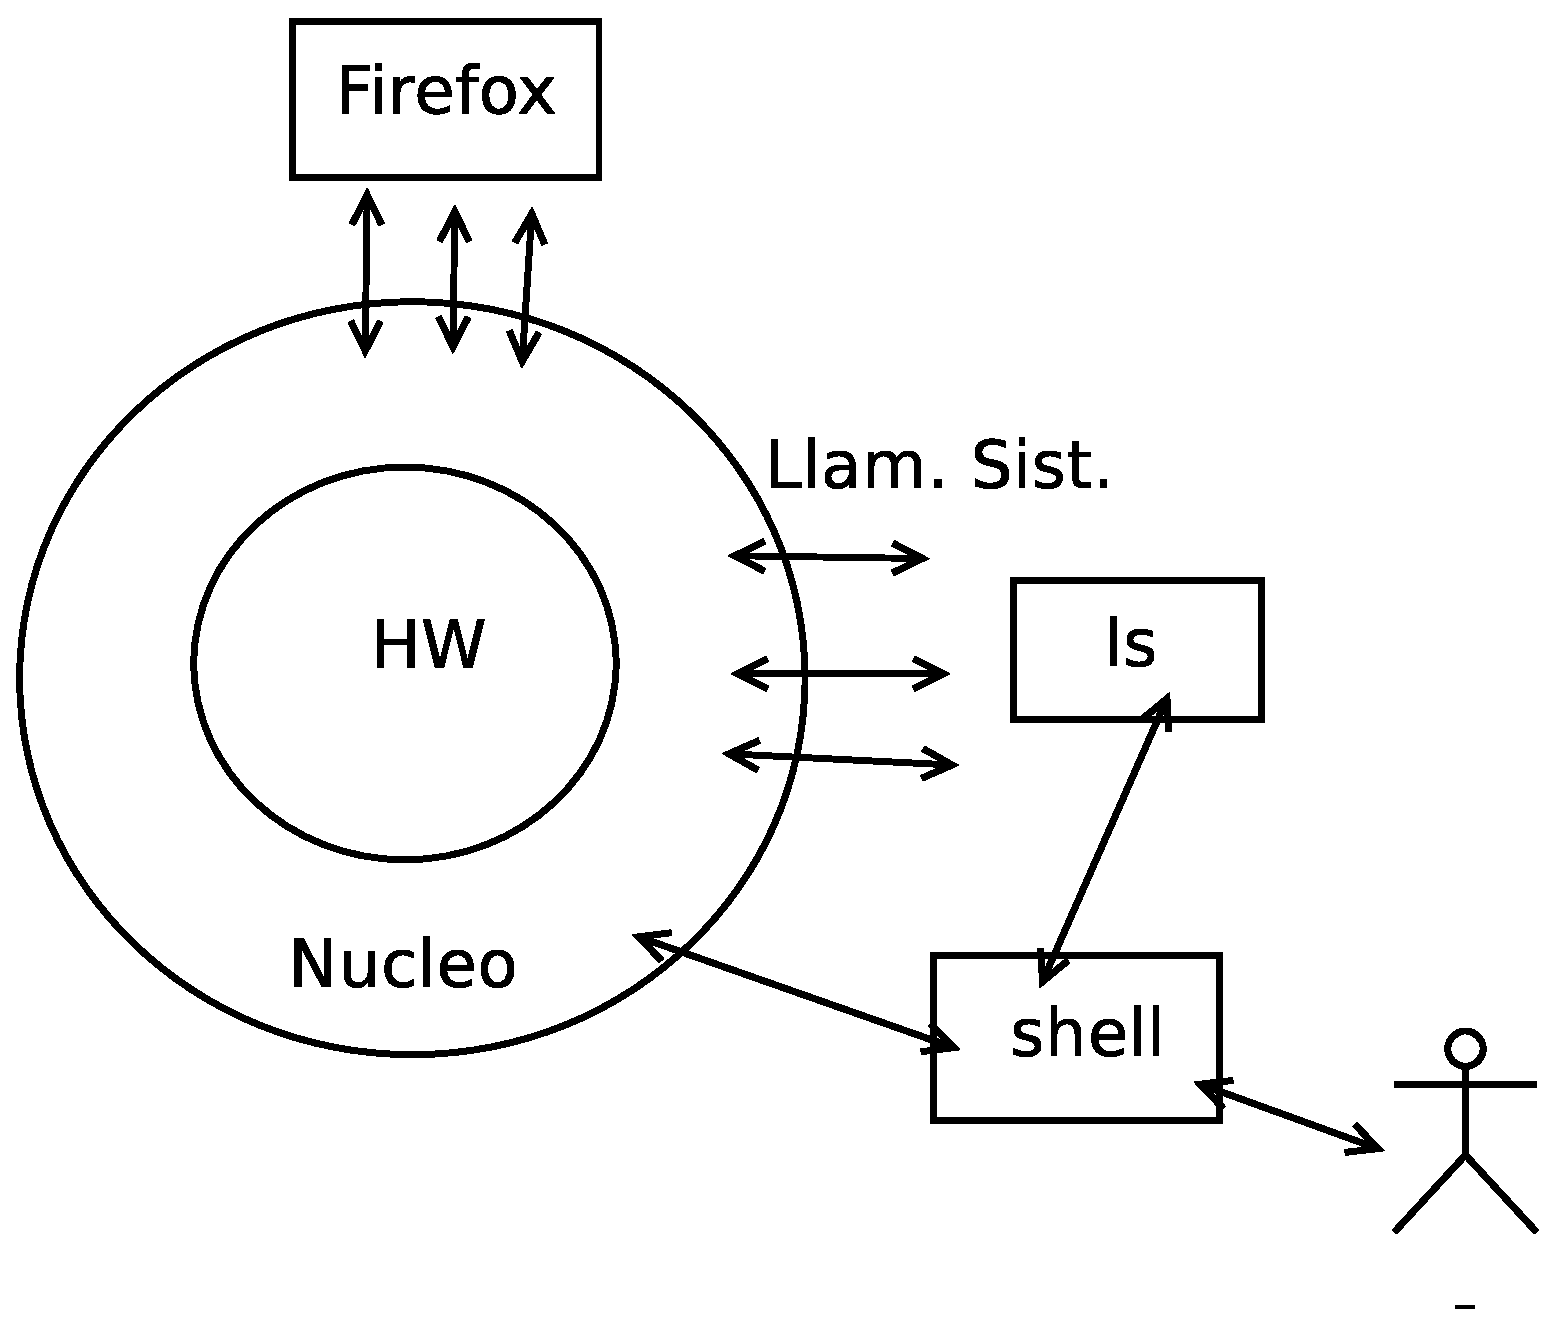
\includegraphics[width=7cm]{figs/nucleo_y_shell}}
\caption{El Sistema Operativo}
\end{figure}
\end{frame}


%%---------------------------------------------------------------
\subsection{¿Quién soy? ¿Dónde estoy? ¿Qué tengo?}
%%---------------------------------------------------------------
\begin{frame}[fragile]
\frametitle{¿Quién soy? ¿Dónde estoy? ¿Qué tengo?}
\begin{itemize}
\item \texttt{whoami}

Muestra el usuario
\item \texttt{id}

Muestra usuario y grupos
\item \texttt{uname \\
uname -a}

Versión de Linux
\item \texttt{hostname}

Nombre de máquina
\item \texttt{pwd}

Directorio de trabajo actual\\
\item \texttt{w}

Usuarios conectados a la máquina
\end{itemize}



\end{frame}
%%---------------------------------------------------------------
\begin{frame}[fragile]

\begin{itemize}


\item

\verb|du       |   Espacio de disco ocupado por los ficheros de un directorio\\
\verb|du -s    |   Espacio de disco ocupado por un directorio\\
\verb|du -h    |   Unidades legibles para un humano\\

\item \texttt{df}

Espacio de disco libre
\end{itemize}
\end{frame}


%%---------------------------------------------------------------
\begin{frame}[fragile]
\begin{itemize} 
\item 

\verb|ls -l    |   Formato largo\\
\verb|ls -a    |   Muestra ficheros ocultos (empiezan por punto)\\
\verb|ls -lh   |   Formato largo, unidades legibles por humano \\
\verb|ls -R    |   Recursivo\\
\verb|ls -ld   |   Lista el directorio, no su contenido\\


\end{itemize}
Unix es \emph{case sensitive}
\end{frame}


%----------------------------------
\subsection{Metacaracteres de la Shell}
%----------------------------------
\begin{frame}[fragile]
\frametitle{Metacaracteres de la Shell}
\begin{itemize} 
\item 
\verb|$      |
Variable 
\item 
\verb|*      |
0 o más caracteres cualquiera
\item 
\verb|?      |
exactamente 1 carácter cualquiera
\item 
\verb|[]     |
1 carácter de la clase
\end{itemize}

ejemplo:

\verb|ls *.txt|

el shell lo expande a 

\verb|ls  texto1.txt texto2.txt texto3.txt|

La orden recibe 3 argumentos, no sabe nada de metacaracteres

\end{frame}


%%---------------------------------------------------
\subsection{Funcionamiento de la shell}
%%---------------------------------------------------


\begin{frame}[fragile]
\frametitle{Funcionamiento (simplificado) de la shell}
La shell:
\begin{enumerate}
\item 
Lee texto de  fichero stdin (por ejemplo, el teclado).
Aporta 
algunas facilidades al usuario (borrar, autocompletar)
\item 
Analiza el texto (expande metacaracteres y variables)
\item 
Toma la primera palabra y busca una orden con ese nombre
en los directorios indicados por PATH

\item
Si puede, 
ejecuta la orden y se queda dormida esperando
a que acabe\\
Por ejemplo

\verb|koji@mazinger:~$ xcalc|

(Mientras usamos la calculadora, la shell permanece inactiva)
\begin{itemize}
\item 
Si queremos que la shell siga activa, 
lanzamos el proceso 
en segundo plano (\emph{background}) \\

\verb|koji@mazinger:~$ xcalc&|

\end{itemize}
\end{enumerate}
\end{frame}

%%---------------------------------------------------------------

%%---------------------------------------------------------------
\begin{frame}[fragile]
\begin{itemize}
\item
Una aplicación lanzada sin \verb|&|, se dice que está
lanzada en primer plano (\emph{foreground}).
\item
La shell se cierra con la orden \verb|exit|. (O con \verb|ctrl d|,
 que representa el fin de fichero)
\end{itemize}

\end{frame}

%%---------------------------------------------------------------
\begin{frame}[fragile]
\frametitle{Autocompletado}
Con frecuencia pasaremos a los mandatos nombres de fichero (como argumento).
La función de autocompletar evita teclear nombres completos

Supongamos que tenemos dos ficheros en el directorio actual


  \begin{footnotesize}
  \begin{verbatim}
.
|-- mi_fichero_del_martes
`-- un_fichero_ejemplo
  \end{verbatim}
  \end{footnotesize}

No es necesario teclear

  \begin{footnotesize}
  \begin{verbatim}
koji@mazinger:~$ ls -l mi_fichero_del_martes
  \end{verbatim}
  \end{footnotesize}

Como solo hay un fichero que empiece por \emph{mi}, basta escribir
  \begin{footnotesize}
  \begin{verbatim}
koji@mazinger:~$ ls -l mi
  \end{verbatim}
  \end{footnotesize}
y luego pulsar tab


\end{frame}

%%---------------------------------------------------------------
%%---------------------------------------------------------------
\begin{frame}[fragile]
Si hay más de un fichero que empiece por \emph{mi}

  \begin{footnotesize}
  \begin{verbatim}
.
|-- mi_fichero_del_martes
|-- mi_fichero_del_miercoles
`-- un_fichero_ejemplo
  \end{verbatim}
  \end{footnotesize}


  \begin{footnotesize}
  \begin{verbatim}
koji@mazinger:~$ ls -l mi_fichero_del_m
mi_fichero_del_martes     mi_fichero_del_miercoles 
  \end{verbatim}
  \end{footnotesize}

Autocompletar rellena hasta donde puede, nos ofrece los ficheros que encajan
en lo que hemos escrito, y espera a que introduzcamos una letra más para
deshacer la ambigüedad (en este ejemplo, \verb|'a'| o \verb|'i'|)

\end{frame}

%%---------------------------------------------------------------
\begin{frame}[fragile]

La shell también autocompleta nombres de ejecutables (si tienen 
permiso de ejecución y están en el path)

  \begin{footnotesize}
  \begin{verbatim}
koji@mazinger:~$ pass<TAB>
  \end{verbatim}
  \end{footnotesize}
Se autocompleta a 
  \begin{footnotesize}
  \begin{verbatim}
koji@mazinger:~$ passwd
  \end{verbatim}
  \end{footnotesize}

De esta manera no hace falta teclear todas las letras. Ni recordar el nombre exacto de órdenes largas, basta saber cómo empiezan

\res{history}

La shell recuerda las últimas
órdenes ejecutadas. Podemos desplazarnos sobre ellas con los cursores
arriba/abajo

\end{frame}







%%---------------------------------------------------------------
\section{Ficheros}
%%---------------------------------------------------------------
\subsection{Árbol de directorios}
%%---------------------------------------------------------------
\begin{frame}[fragile]
\frametitle{Árbol de directorios}
\begin{minipage}{4.5cm}
\begin{figure}
\centerline{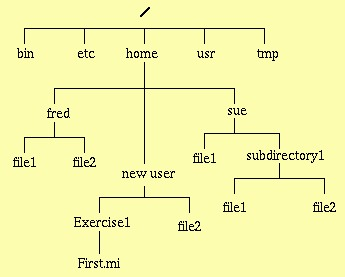
\includegraphics[width=4.5cm]{figs/unix-tree}}
\end{figure}
\end{minipage} \hfill
\
\begin{minipage}{4.5cm}
\begin{itemize} 
\item Árbol, todo cuelga de un único directorio raiz
\item Dentro de cada directorio, habrá ficheros o subdirectorios
\item jerarquía clásica unix:
        \begin{itemize}
        \item /home
        \item /bin
        \item /usr
        \item   (...)
        \end{itemize}
\end{itemize}
\end{minipage} \hfill
\end{frame}


%--------------------------------------------------------------------

\begin{frame}[fragile]

\frametitle{Nombres de fichero}
  \begin{itemize}
    \item Hasta 256 caracteres
    \item Mayúsculas y minúsculas son distintas
          \begin{itemize}
          \item Se puede tener en un mismo directorio los ficheros
                   \verb|ejemplo|, \verb|EJEMPLO| y \verb|EjemPlO|
          \item Pero si llevamos estos ficheros a una unidad externa
            (pendrive, disco) que mantenga su formato por omisión
             (FAT32), deja de ser legal
          \end{itemize}
    % \item Los que empiezan por punto (\verb|.|) se consideran ocultos
    \item
Los que empiezan por punto (\verb|.|)se consideran ocultos
    (por defecto no se muestran), suelen usarse para ficheros o
    directorios de configuración
    \item Casi cualquier carácter es legal, pero es preferible usar solo números, letras, guión y barra baja. 
  \begin{itemize}
    \item Es preferible evitar los espacios
   \item También es buena idea evitar eñes y tildes (Naturalmente, hablamos del nombre del fichero, no de su contenido)
  \end{itemize}
  
%
%    \item Es preferible evitar los caracteres: espacio \verb| dolar ? \ *|
  \end{itemize}
\end{frame}





%%---------------------------------------------------------------
\subsection{Permisos}
%%---------------------------------------------------------------

%\begin{frame}[fragile]
%  \begin{itemize}
%  \item Unix es un sistema operativo multiusuario.
%  \item Los usuarios se reparten en \res{grupos} de usuarios.
%    \begin{itemize}
%    \item Un usuario puede pertenecer a varios grupos.
%    \item Todo usuario pertenece a un grupo principal      
%    \end{itemize}
%  \item Cada usuario tiene asociado:
%    \begin{itemize}
%    \item un identificador numérico de usuario: \res{UID} (\emph{user id}).
%    \item un identificador númerico de grupo: \res{GID} (\emph{group id}).
%    \end{itemize}
%  \item Identificadores de texto asocian:
%    \begin{itemize}
%    \item a cada UID un nombre de usuario (login)
%    \item a cada GID un nombre de grupo
%    \end{itemize}
%  \end{itemize}
%\end{frame}

%%-------------------------------------------------------
%
%\begin{frame}[fragile]
%  \section{Mandatos}
%  \begin{itemize}
%  \item \res{whoami}: Muestra el login del usuario.
%    \begin{footnotesize}
%      \begin{tabbing}
%        \verb|echo hola|\hspace{1cm} \= No escribe nada útil aquí\kill
%        \verb|whoami| \> \\
%      \end{tabbing}
%    \end{footnotesize}
%  \item \res{id}: Muestra información sobre el usuario
%    \begin{footnotesize}
%      \begin{tabbing}
%        \verb|echo hola|\hspace{1cm} \= No escribe nada útil aquí\kill
%        \verb|id| \>  Muestra UID (y login), GID (y nombre de grupo),
%        y lista de otros\\\> grupos a los que pertenece el usuario\\
%        \verb|id -un| \>  Idéntico a \verb|whoami|\\
%      \end{tabbing}
%    \end{footnotesize}
%  \item \res{who}: Muestra qué usuarios están conectados
%    \begin{footnotesize}
%      \begin{tabbing}
%        \verb|echo hola|\hspace{1cm} \= No escribe nada útil aquí\kill
%        \verb|who| \> \\
%      \end{tabbing}
%    \end{footnotesize}
%  \item \res{w}: Muestra qué usuarios están conectados, incluyendo
%    información del sistema
%    \begin{footnotesize}
%      \begin{tabbing}
%        \verb|echo hola|\hspace{1cm} \= No escribe nada útil aquí\kill
%        \verb|w| \> 
%      \end{tabbing}
%    \end{footnotesize}
%  \end{itemize}
%\end{frame}

%%%-------------------------------------------------------
%
%\begin{frame}[fragile]
%
%  \begin{itemize}
%  \item \res{finger}: Muestra información sobre usuarios.
%    \begin{footnotesize}
%      \begin{tabbing}
%        \verb|finger jose@maquina| \= No escribe nada útil aquí\kill
%        \verb|finger| \> Muestra qué usuarios están conectados\\
%        \verb|finger jose| \> Muestra información sobre el usuario
%        \verb|jose| (si existe) o sobre\\\> cualquier usuario que tenga
%        \verb|jose| como parte de su login o de \\\>su nombre completo\\
%        \> Incluye el contenido de sus
%        ficheros \verb|.plan|, \verb|.project|,\\\> \verb|.pgpkey| y
%        \verb|.forward|, si existen.\\                   
%        \verb|finger jose@maquina| \> Busca entre los usuarios de la
%        máquina \verb|maquina|.\\\> La mayoría de máquinas hoy suelen
%        tener deshabilitado este\\\> servicio por razones de seguridad.
%      \end{tabbing}
%    \end{footnotesize}
%  \end{itemize}
%
%\end{frame}


%%-------------------------------------------------------

\begin{frame}[fragile]
  \frametitle{Permisos}
  \res{ls -l}: Muestra los contenidos de los directorios en
    \textbf{formato largo}:
\begin{verbatim}
drwxr-xr-x 2 jperez al-07-08 4096 2007-10-09 22:51 d1
-rw-r--r-- 1 jperez al-07-08 8152 2007-10-16 09:42 f1
-rw-r--r-- 1 jperez al-07-08   24 2007-10-16 09:42 f3
\end{verbatim}


% http://tldp.org/LDP/intro-linux/html/sect_03_01.html
El primer carácter indica:

  \begin{footnotesize}
  \begin{verbatim}
-       Regular file - Fichero ordinario
d       Directory - Directorio
l       (Symbolic) Link - Enlace simbólico
p       Named pipe - Pipe con nombre
s       Socket - Socket
c       Character device - Dispositivo orientado a carácter
b       Block device - Dispositivo orientado a bloque
  \end{verbatim}
  \end{footnotesize}
% character device: un chorro de bytes, acceso secuencial,
% como un terminal

% dispotivo de bloques: acceso aleatorio, como un disco

\end{frame}
%%----------------------------------------------
\begin{frame}[fragile]

    Para cada entrada, aparece, además:
    \begin{footnotesize}
      \begin{itemize}
      \item \res{permisos}: Los 10 primeros caracteres
      \item número de nombres del fichero (enlaces duros)
      \item \res{usuario del dueño}
      \item \res{grupo del dueño}
      \item tamaño en bytes
      \item fecha y hora de la última modificación
      \item nombre
      \end{itemize}
    \end{footnotesize}
\end{frame}

%%-------------------------------------------------------
\begin{frame}[fragile]

  \begin{center}
  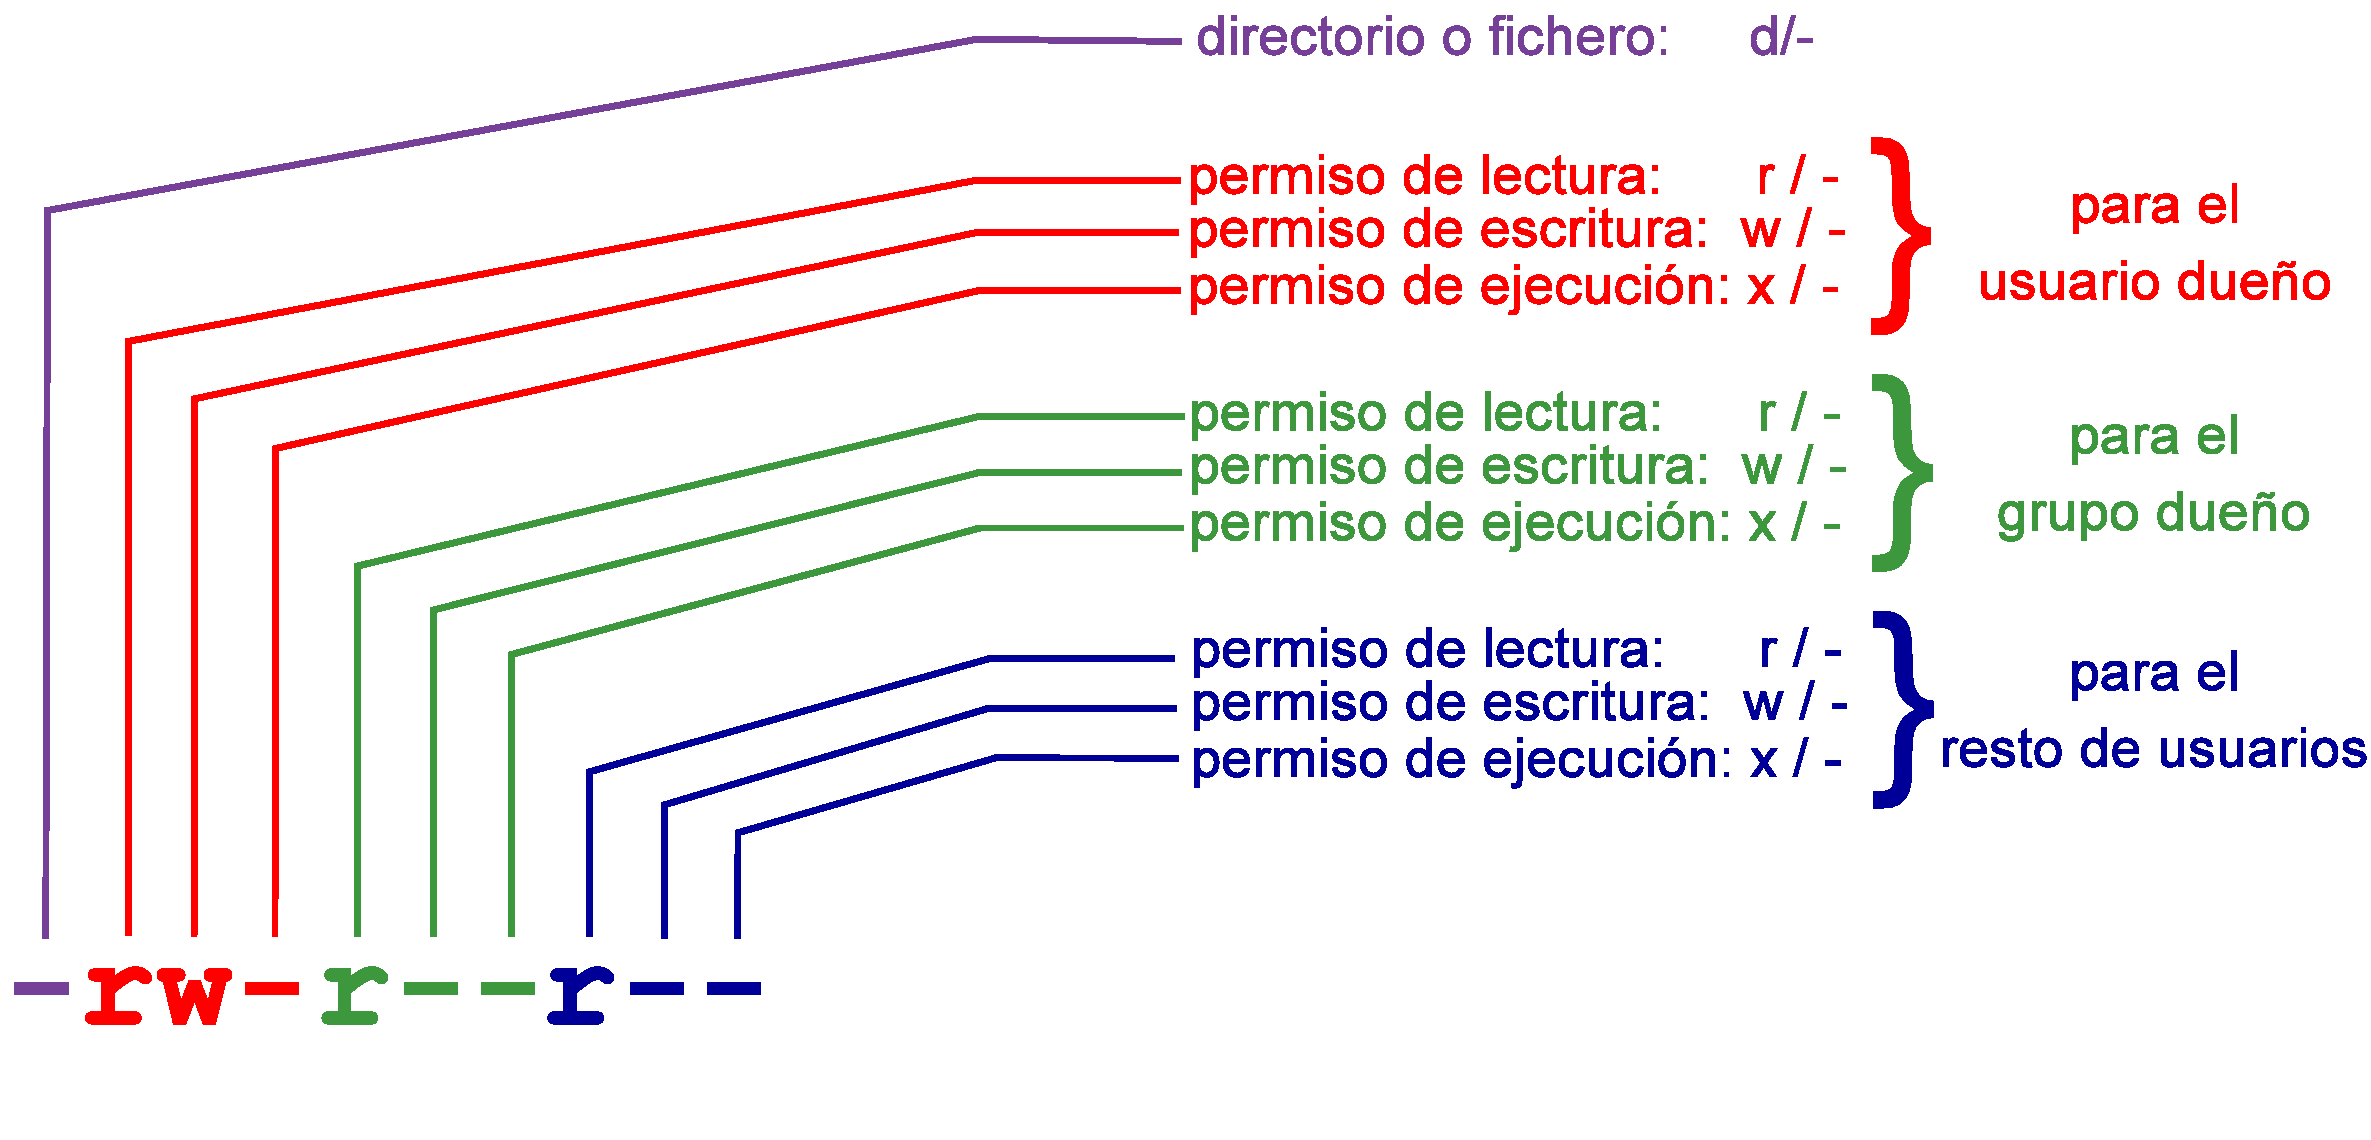
\includegraphics[width=\textwidth]{figs/unix-mode}
  \end{center}

  NOTA: En inglés, al conjunto de permisos de un fichero se le
  conoce como el ``modo de acceso'' (\emph{access mode}).

\end{frame}

\begin{frame}[fragile]

%  \begin{footnotesize}
    \begin{itemize}
    \item \res{Permisos de un fichero}:
      \begin{itemize}
      \item El de \textbf{lectura}: permite ver su contenido
      \item El de \textbf{escritura}: permite modificar su contenido
      \item El de \textbf{ejecución}: permite ejecutarlo
      \end{itemize}
    \item \res{Permisos de un directorio}:
      \begin{itemize}
      \item El de \textbf{lectura}: permite hacer \verb|ls| del contenido
      \item El de \textbf{escritura}: permite crear y borrar
        ficheros y subdirectorios dentro de él
      \item El de \textbf{ejecución}: permite hacer \verb|cd| a él
      \end{itemize}
      \end{itemize}
    \begin{tabbing}
      Permisos \emph{normales} de un directorio: \= \verb|drwxr-xr-x|\kill
      Permisos \emph{normales} de un fichero: \> \verb|-rw-r--r--|\\
      Permisos \emph{normales} de un directorio: \> \verb|drwxr-xr-x|
    \end{tabbing}    
%  \end{footnotesize}

\end{frame}


%%%-------------------------------------------------------
%\begin{frame}[fragile]
%
%  \begin{itemize}
%  \item \res{chmod}: Cambia los permisos de un fichero (\emph{change mode})\\
%    \vspace{-2mm}\\\textbf{SINTAXIS 1}: \verb|chmod [ugoa][+-][rwx] <elem1> <elem2> ...|
%    \begin{footnotesize}
%      \begin{tabbing}
%        a\hspace{4mm} \= \verb|ugoa|\hspace{2mm} \= \kill
%        \> \verb|ugoa| \> permisos para el usuario(\verb|u|)/grupo(\verb|g|)/resto(\verb|o|)/todos(\verb|a|)\\
%        \> \verb|+-| \> pone(\verb|+|)/quita(\verb|-|) el permiso\\
%        \> \verb|rwx| \> permiso de lectura(\verb|r|)/escritura(\verb|w|)/ejecución(\verb|x|)
%      \end{tabbing}
%    \end{footnotesize}
%
%    \begin{footnotesize}
%      \begin{tabbing}
%        \verb|echo hola|\hspace{2.2cm} \= No escribe nada útil aquí\kill
%        \verb|chmod u+rw f1| \> Añade permisos r, w para el usuario dueño\\
%        \verb|chmod a-w f1| \> Quita permiso w a todos\\
%        \verb|chmod u+rw,g-w,o-w f1| \> Varios grupos de opciones
%        pueden separarse por comas\\
%        \verb|chmod -R a+r d1| \> Con \verb|-R| opera también
%        recursivamente sobre los contenidos\\\> del directorio
%      \end{tabbing}
%    \end{footnotesize}
%  \end{itemize}
%
%\end{frame}

%%%-------------------------------------------------------
%\begin{frame}[fragile]
%
%  \begin{itemize}
%  \item \res{chmod}: Cambia los permisos de un fichero (\emph{change mode})\\
%    \vspace{-2mm}\\\textbf{SINTAXIS 2}: \verb|chmod <modo-en-octal> <elem1> <elem2> ...|
%    \begin{footnotesize}
%      \begin{tabbing}
%        a\hspace{2mm} \= \verb|ugoa|\hspace{22mm} \= \kill
%        \> \verb|<modo-en-octal>| \> 3 cifras octales (0-7), cada una
%        represantando el valor resultante\\\>\> de considerar cada grupo de
%        3 permisos un número binario,\\\>\> siendo 1 el permiso
%        activado y 0 el permiso quitado
%      \end{tabbing}
%    \end{footnotesize}
%
%    \begin{footnotesize}
%      \begin{tabbing}
%        \verb|echo hola|\hspace{1cm} \= No escribe nada útil aquí\kill
%        \verb|chmod 644 f1| \> Pone permisos \verb|rw-r--r--| a \verb|f1|\\ 
%        \verb|chmod 755 d1| \> Pone permisos \verb|rwxr-xr-x| a \verb|d1|\\
%        \verb|chmod 600 f1| \> Pone permisos \verb|rw-------| a \verb|f1|\\
%     \end{tabbing}
%    \end{footnotesize}
%  \end{itemize}
%
%\end{frame}


%%-------------------------------------------------------
%
%\begin{frame}[fragile]
%  \section{Usuario root}
%  \begin{itemize}
%  \item El usuario de UID 0 es el superusuario
%  \item Su login es normalmente \verb|root|
%  \item A él no se le aplican los permisos de los ficheros, siempre
%    puede leer, escribir o ejecutar un fichero o directorio
%  \item Es peligroso trabajar como \verb|root|: debe reservarse para
%    lo estrictamente imprescindible.
%  \end{itemize}
%\end{frame}



%%-------------------------------------------------------
%
%
%\begin{frame}[fragile]
%
%  \begin{itemize}
%  \item \res{chown}: Cambia el usuario dueño de un fichero
%    (\emph{change owner}). Sólo puede invocarlo el usuario \verb|root|
%    \begin{footnotesize}
%      \begin{tabbing}
%        \verb|echo hola|\hspace{3cm} \= No escribe nada útil aquí\kill
%        \verb|chown pepe f1| \> \\
%        \verb|chown pepe.al-07-08 f1| \> Cambia también el grupo dueño
%      \end{tabbing}
%    \end{footnotesize}
%  \item \res{chgrp}: Cambia el grupo dueño de un fichero
%    (\emph{change group}). Sólo puede invocarlo el usuario \verb|root|
%    \begin{footnotesize}
%      \begin{tabbing}
%        \verb|echo hola|\hspace{1cm} \= No escribe nada útil aquí\kill
%        \verb|chgrp al-07-08 f1| \> 
%      \end{tabbing}
%    \end{footnotesize}
%  \end{itemize}
%
%\end{frame}
%



% \begin{frame}[fragile]

%   \begin{itemize}
%   \item \res{fortune}: Muestra un pensamiento al azar.
%     \begin{footnotesize}
%       \begin{tabbing}
%         \verb|echo hola|\hspace{1cm} \= No escribe nada útil aquí\kill
%         \verb|fortune| \> \\
%         \verb|fortune| \> \\
%         \verb|fortune| \> \\
%         \verb|fortune| \> \\
%       \end{tabbing}
%     \end{footnotesize}
%   \end{itemize}

% \end{frame}


% Local Variables: 
% mode: latex
% TeX-master: "intro-shell-main"
% End: 




\begin{frame}[fragile]
\frametitle{Cambio de permisos}
\begin{minipage}{7cm}
\begin{figure}
\centerline{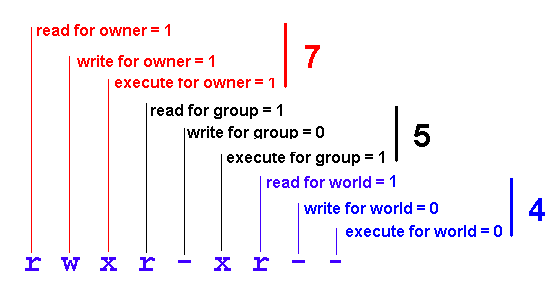
\includegraphics[width=7cm]{figs/permission}}
\end{figure}
\end{minipage} \hfill
\

\begin{itemize}
\item
Los permisos se representan con una secuencia de caracteres: r,w,x
(lectura, escritura y ejecución)
\item
Un guión indica la ausencia del permiso correspondiente a esa posición
\end{itemize}
\end{frame}



%%---------------------------------------------------------------
\begin{frame}[fragile]
\frametitle{}
Para cambiar permisos se usa \verb|chmod|, que tiene dos sintaxis
equivalentes, se puede usar la que resulte más cómoda
\begin{enumerate} 
\item 
\verb|chmod  754 mi_fichero|

No importan los permisos que tuviera previamente el fichero,
pasa a tener:

  \begin{footnotesize}
  \begin{verbatim}
  7   5   4        (octal)
111 101 100        (binario)
rwx r-x r--
  \end{verbatim}
  \end{footnotesize}

\item 
\verb|chmod [ugo] [+-] [rwx] mi_fichero| \\
\verb|chmod o+x mi_fichero|

A partir de los permisos que tuviera el fichero, se suman o
se restan los permisos indicados a u,g,o  (user, group, other)
\end{enumerate}

\end{frame}


%%---------------------------------------------------------------
\begin{frame}[fragile]
\begin{itemize}
\item
Para la primera forma, es necesario saber contar en binario
hasta 7
 
\begin{verbatim}
   Octal   Binario
   ----------------
     0     000
     1     001
     2     010
     3     011
     4     100
     5     101
     6     110
     7     111
\end{verbatim}
\end{itemize}

\end{frame}



%%---------------------------------------------------------------
\begin{frame}[fragile]
\frametitle{Permisos de los directorios}
\verb|chmod -R |   Cambia permisos recursivamente
\begin{itemize} 
\item 
\texttt{r} y  
\texttt{x} normalmente van juntos. (Ambos o ninguno).

Permiten entrar en el directorio y listar
\item \texttt{w} permite añadir añadir ficheros o borrarlos
\end{itemize}

\textcolor{red}{Muy Importante}:\\Comprueba los permisos de tu \verb|HOME|, en muchos sistemas por omisión está abierto

\textcolor{red}{Atención},\\un fichero sin permisos de escritura, p.e. \verb|rwxr-xr-x|\\
pero con permiso de escritura en el directorio que lo contiene, \verb|rwxrwxrwx|\\
no podrá ser modificado pero sí borrado o renombrado

\begin{scriptsize}
%(a menos que esté el \emph{sticky bit} activado 
%\verb|   chmod [+-]t dir|)
\end{scriptsize}
\end{frame}

%%---------------------------------------------------------------



%%---------------------------------------------------------------
\subsection{path}
%%---------------------------------------------------------------


\begin{frame}[fragile]
  \frametitle{Directorios Especiales}

  \begin{itemize}
  \item Todo directorio contiene dos subdirectorios especiales:
    \begin{footnotesize}
      \begin{tabbing}
        \verb|echo -n|\hspace{3mm} \= No escribe nada útil aquí\kill
        \verb|.| \> El subdirectorio \verb|.| de un directorio es él mismo\\
        \verb|..| \> El subdirectorio \verb|..| de un directorio es su
        directorio padre\\
      \end{tabbing}
    \end{footnotesize}
  \end{itemize}
  \begin{minipage}{5cm}
    ~\hspace{-1cm}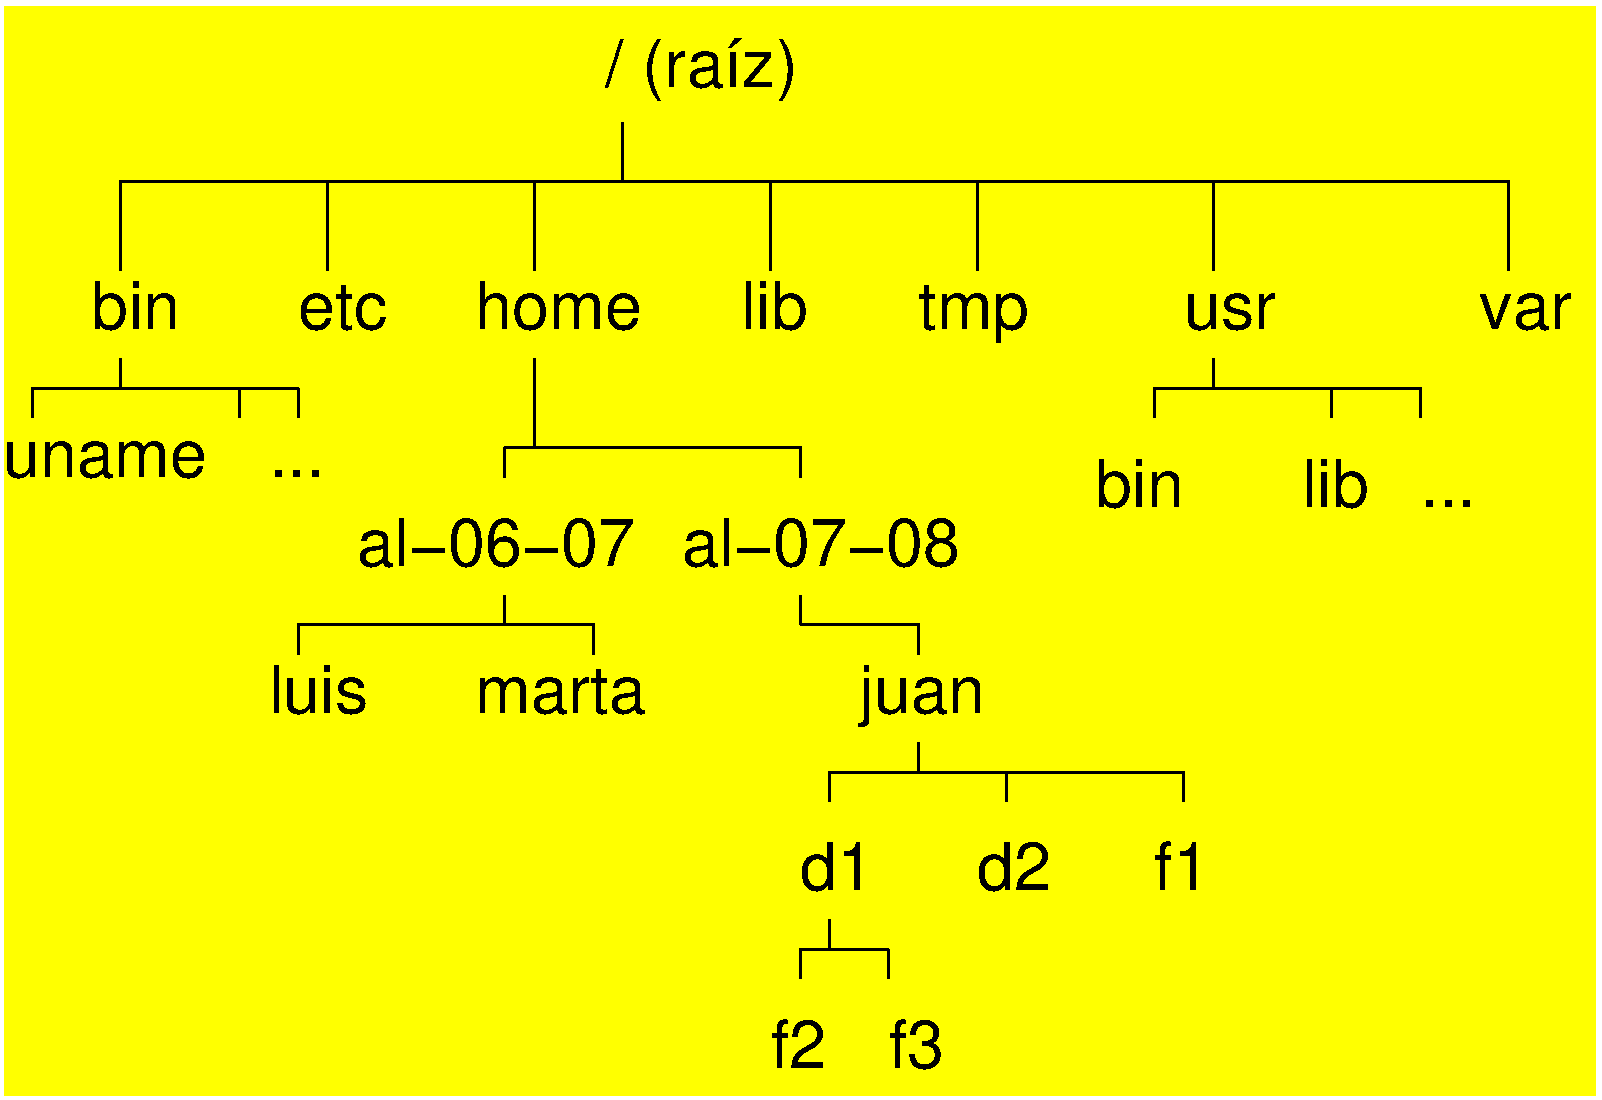
\includegraphics[width=5cm]{figs/unix-tree-2}
  \end{minipage}
  \begin{minipage}{5.0cm}
  \begin{itemize}
  \item Ejemplos:
    \begin{footnotesize}
      \begin{itemize}
      \item El subdirectorio \verb|.| de \verb|al-07-08| es \verb|al-07-08|
      \item El subdirectorio \verb|..| de \verb|al-07-08| es \verb|home|
      \item El subdirectorio \verb|..| de \verb|home| es \verb|/|
      \end{itemize}
    \end{footnotesize}    
  \end{itemize}
  \end{minipage}

\end{frame}




%%---------------------------------------------------------------
\section{Variables}
%%---------------------------------------------------------------

\begin{frame}[fragile]
\frametitle{Variables }
\begin{itemize} 
\item  \verb|variable=valor|\\
\verb|echo $variable| \\
Sin espacios antes y despues del igual\\
con \$ para acceder al contenido de la variable\\
sin \$ en la asignación\\
sólo son visibles en ese proceso
\end{itemize}
\begin{footnotesize}
\begin{verbatim}
nombre=juan 
echo $nombre
\end{verbatim}
\end{footnotesize}


\end{frame}
%%---------------------------------------------------------------
\begin{frame}[fragile]
\subsection{Variables de entorno}

\frametitle{Variables de entorno}
\begin{itemize} 
\item
\verb|export VARIABLE=valor|\\hace que los procesos hijos del proceso donde 
se declara la variable, la reciban. Por convenio se usan mayúsculas

%% ojo al probar esto, se puede hacer una demo con xterm
%% pero no con gnome-terminal, puesto que si desde
%% un gnome-terminal lanzo otro, el segundo no es hijo
%% del primero, debe ser el mismo proceso

\item
Para que el cambio sea permanente, hay que exportar la variable
en algún fichero de configuración como p.e.
\verb|.bashrc|


\item \verb|printenv| \\muestra todas las variables de entorno
\item 
HOME  
\item 
HOSTNAME 
\item 
USER 
\item PATH\\
Contiene la lista de directorios donde la shell buscará los
ejecutables (si no se indica path explícito)
%\texttt{export PATH=\$PATH:/usr/local/bin:.}
%%\item PS1
\end{itemize}
\end{frame}

%%---------------------------------------------------------------
\begin{frame}[fragile]
\frametitle{La variable de entorno HOME}
\begin{itemize}
\item
Indica el directorio \emph{hogar} de un usuario: el sitio donde se espera
que cada usuario escriba sus cosas
\begin{footnotesize}
\begin{verbatim}
koji@mazinger:~$ echo $HOME
/home/koji
\end{verbatim}
\end{footnotesize}
\item
Se le suele llamar \verb|$HOME|, pero esto no es muy preciso
\begin{itemize}
\item La variable se llama \verb|HOME|, el dólar se antepone a todas
las variables en bash cuando se están referenciando (y no cuando se asignan)
\item Es un error frecuente intentar usar \verb|$HOME| en otros lenguajes
o en cualquier programa. Solo es válido en bash y shells similares
\end{itemize}
\end{itemize}

\end{frame}


%%---------------------------------------------------------------

%%---------------------------------------------------------------
\begin{frame}[fragile]
\frametitle{Virgulilla}
La virgulilla (\verb|~|) representa el directorio \emph{home} de un usuario
\begin{itemize}
\item
Equivale a \verb|$HOME|, con la ventaja de que se puede usar en
muchos lenguajes, aplicaciones y librerías (no todos)
\item
No aparece en los teclados, pero está accesible en \verb|AltGr 4|
\item
Seguida de un nombre de usuario, representa el \emph{HOME} de ese usuario
\begin{footnotesize}
\begin{verbatim}
koji@mazinger:~$ echo ~jperez
/home/jperez
\end{verbatim}
\end{footnotesize}

\end{itemize}

\end{frame}

%%---------------------------------------------------------------
\begin{frame}[fragile]
Si el nombre del usuario no es una cadena literal sino una variable
es necesario volver a evaluar la expresión

  \begin{footnotesize}
  \begin{verbatim}
koji@mazinger:~$ nombre=koji
koji@mazinger:~$ echo ~$nombre
~koji
koji@doublas:~$ eval echo ~$nombre
/home/koji
  \end{verbatim}
  \end{footnotesize}


\end{frame}



%%---------------------------------------------------------------
\begin{frame}[fragile]
\subsection{La variables de entorno PATH}
\frametitle{La variable de entorno PATH}
Un usuario principiante ejecuta
\begin{footnotesize}
\begin{verbatim}
koji@mazinger:~/pruebas$ ls -l
total 4
-rw-r--r-- 1 koji koji 27 2009-10-07 19:02 holamundo
\end{verbatim}
\end{footnotesize}
Intenta invocar el mandato \emph{holamundo} escribiendo
\begin{footnotesize}
\begin{verbatim}
koji@mazinger:~/pruebas$ holamundo
\end{verbatim}
\end{footnotesize}
pero obtiene
\begin{footnotesize}
\begin{verbatim}
bash: holamundo: orden no encontrada
\end{verbatim}
\end{footnotesize}
\end{frame}



%%---------------------------------------------------------------
\begin{frame}[fragile]
\res{Problema 1}

 El fichero no tenía permisos de ejecución

\res{Problema 1: Solución }
\begin{footnotesize}
\begin{verbatim}
koji@mazinger:~/pruebas$ chmod ugo+x holamundo
\end{verbatim}
\end{footnotesize}

¿Problema resuelto?
\begin{footnotesize}
\begin{verbatim}
koji@mazinger:~/pruebas$ ls -l
total 4
-rwxr-xr-x 1 koji koji 27 2009-10-07 19:02 holamundo
\end{verbatim}
\end{footnotesize}


No ha bastado. El usuario vuelve a ejecutar
\begin{footnotesize}
\begin{verbatim}
koji@mazinger:~/pruebas$ holamundo
\end{verbatim}
\end{footnotesize}
pero vuelve a obtener
\begin{footnotesize}
\begin{verbatim}
bash: holamundo: orden no encontrada
\end{verbatim}
\end{footnotesize}
\end{frame}



%%---------------------------------------------------------------
\begin{frame}[fragile]
\res{Problema 2}

Aunque el fichero está en el directorio actual (directorio \emph{punto}),
la shell no lo buscará allí, sino donde indique la variable 
de entorno PATH, que contiene una lista de directorios, separados 
por el carácter
\emph{dos puntos} 

\begin{footnotesize}
\begin{verbatim}
koji@mazinger:~/pruebas$ echo $PATH
/usr/local/sbin:/usr/local/bin:/usr/sbin:/usr/bin:/sbin:/bin
\end{verbatim}
\end{footnotesize}

Lo buscará en 
\verb|/usr/local/sbin|

Si no lo encuentra, lo buscará en
\verb|/usr/local/bin|

Si sigue sin encontrarlo, lo buscará en
\verb|/usr/local/sbin|

etc

Pero no lo buscará en el directorio \emph{punto}

\end{frame}



%%---------------------------------------------------------------
\begin{frame}[fragile]
\res{Problema 2: Solución 1 (recomendada)}


Invocar el mandato indicando explícitamente que el fichero
está en el directorio \emph{punto}
\begin{footnotesize}
\begin{verbatim}
koji@mazinger:~/pruebas$ ./holamundo 
¡hola mundo!
\end{verbatim}
\end{footnotesize}



\res{Problema 2: Solución 2}

Indicar el trayecto absoluto del mandato


\begin{footnotesize}
\begin{verbatim}
koji@mazinger:~/pruebas$ /home/koji/pruebas/holamundo 
¡hola mundo!
\end{verbatim}
\end{footnotesize}


\begin{footnotesize}
\begin{verbatim}
\end{verbatim}
\end{footnotesize}


\begin{footnotesize}
\begin{verbatim}
\end{verbatim}
\end{footnotesize}


\end{frame}


%%---------------------------------------------------------------
\begin{frame}[fragile]
\res{Problema 2: Solución 3}

Modificamos la variable de entorno PATH para añadir \res{al final} el
directorio \emph{punto}

Como queremos que el cambio sea permanente, debemos modificar 
la variable en un fichero de configuración
\footnote{Más detalles en el apartado \emph{invocación de la shell}}
, por ejemplo  \verb|~/.bashrc|

\begin{footnotesize}
\begin{verbatim}
export PATH=$PATH:.
\end{verbatim}
\end{footnotesize}

El cambio no se produce de inmediato, sino cuando se ejecute de nuevo 
 \verb|~/.bashrc|
\begin{itemize}
\item 
Al invocarlo explícitamente

\begin{footnotesize}
\begin{verbatim}
koji@mazinger:~/pruebas$ source ~/.bashrc
\end{verbatim}
\end{footnotesize}
\item
Al abrir una nueva terminal
\end{itemize}
\end{frame}

%%---------------------------------------------------------------
\begin{frame}[fragile]
\res{Problema 2: Solución 4 ¡Muy peligrosa!}

Modificamos la variable de entorno PATH para añadir \res{al principio} el
directorio \emph{punto}

\verb|export PATH=.:$PATH|

Supongamos que un atacante escribe un script con el nombre \verb|ls| 
y el contenido  
\begin{footnotesize}
\begin{verbatim}
#!/bin/bash
rm -rf  $HOME
\end{verbatim}
\end{footnotesize}

Al escribir la orden \verb|ls|, se ejecutaría este script, y no \verb|/bin/ls|

\begin{footnotesize}
\begin{verbatim}
\end{verbatim}
\end{footnotesize}



\end{frame}





%%---------------------------------------------------------------

\begin{frame}[fragile]
  \frametitle{Directorio de Trabajo}

  \begin{itemize}
  \item La shell en todo momento se encuentra en un cierto punto del
    árbol de ficheros. A ese punto se le llama \textbf{directorio de trabajo}
 (\emph{working directory})
  \item Normalmente la shell indica el directorio de trabajo en el \emph{prompt}
  \item pwd: Muestra el directorio de trabajo actual
    (\emph{print working directory})
    \begin{footnotesize}
      \begin{tabbing}
        \verb|echo -n hola a todos|\hspace{1cm} \= No escribe nada útil aquí\kill
        \verb|pwd| \> \\
      \end{tabbing}
    \end{footnotesize}
  %\item En las páginas siguientes, DT significa ``directorio de trabajo''.
  \end{itemize}

\end{frame}

%%---------------------------------------------------------------

\begin{frame}[fragile]
  \frametitle{Trayectos (Paths)}

  \begin{itemize}
  \item Un trayecto (path) consiste en escribir el camino hasta un
    fichero o directorio, incluyendo directorios intermedios separados
    por el carácter \verb|/|
  \item Trayecto absoluto: 
    \begin{footnotesize}
      \begin{itemize}
      \item Escribe el camino desde el \textbf{directorio raíz}
      \item \textbf{Siempre} empieza por \verb|/|
      \end{itemize} 
    \end{footnotesize}
  \item Trayecto relativo: 
    \begin{footnotesize}
      \begin{itemize}
      \item Escribe el camino desde el directorio de trabajo
      \item \textbf{Nunca} empieza por \verb|/|
      \end{itemize} 
    \end{footnotesize}


\item
Cualquier programa acepta (o debería aceptar) que cuando
se especifica un nombre de fichero, se use o bien la forma
relativa o bien la forma absoluta. 

Esto es aplicable a casi cualquier programa de casi
cualquier Sistema Operativo

  \end{itemize}

\end{frame}



%%---------------------------------------------------------------
\begin{frame}[fragile]
%\frametitle{}
¿Un trayecto con virgulilla es relativo o absoluto?

\verb|~/mi_directorio|

En cierta forma es relativo
\begin{itemize}
\item
No empieza por \verb|/|
\item
Depende del usuario que lo ejecuta
\end{itemize}

En cierta forma es absoluto
\begin{itemize}
\item
No depende del directorio de trabajo
\item
Lo que sucede realmente es que se reemplaza la virgulilla por el trayecto
absoluto del \emph{home} del usuario
\end{itemize}

Posiblemente lo más adecuado es considerarlo un caso un poco
especial de \res{path absoluto}


\end{frame}
%%---------------------------------------------------------------


\begin{frame}[fragile]

  \begin{minipage}{4cm}
    ~\hspace{-1cm}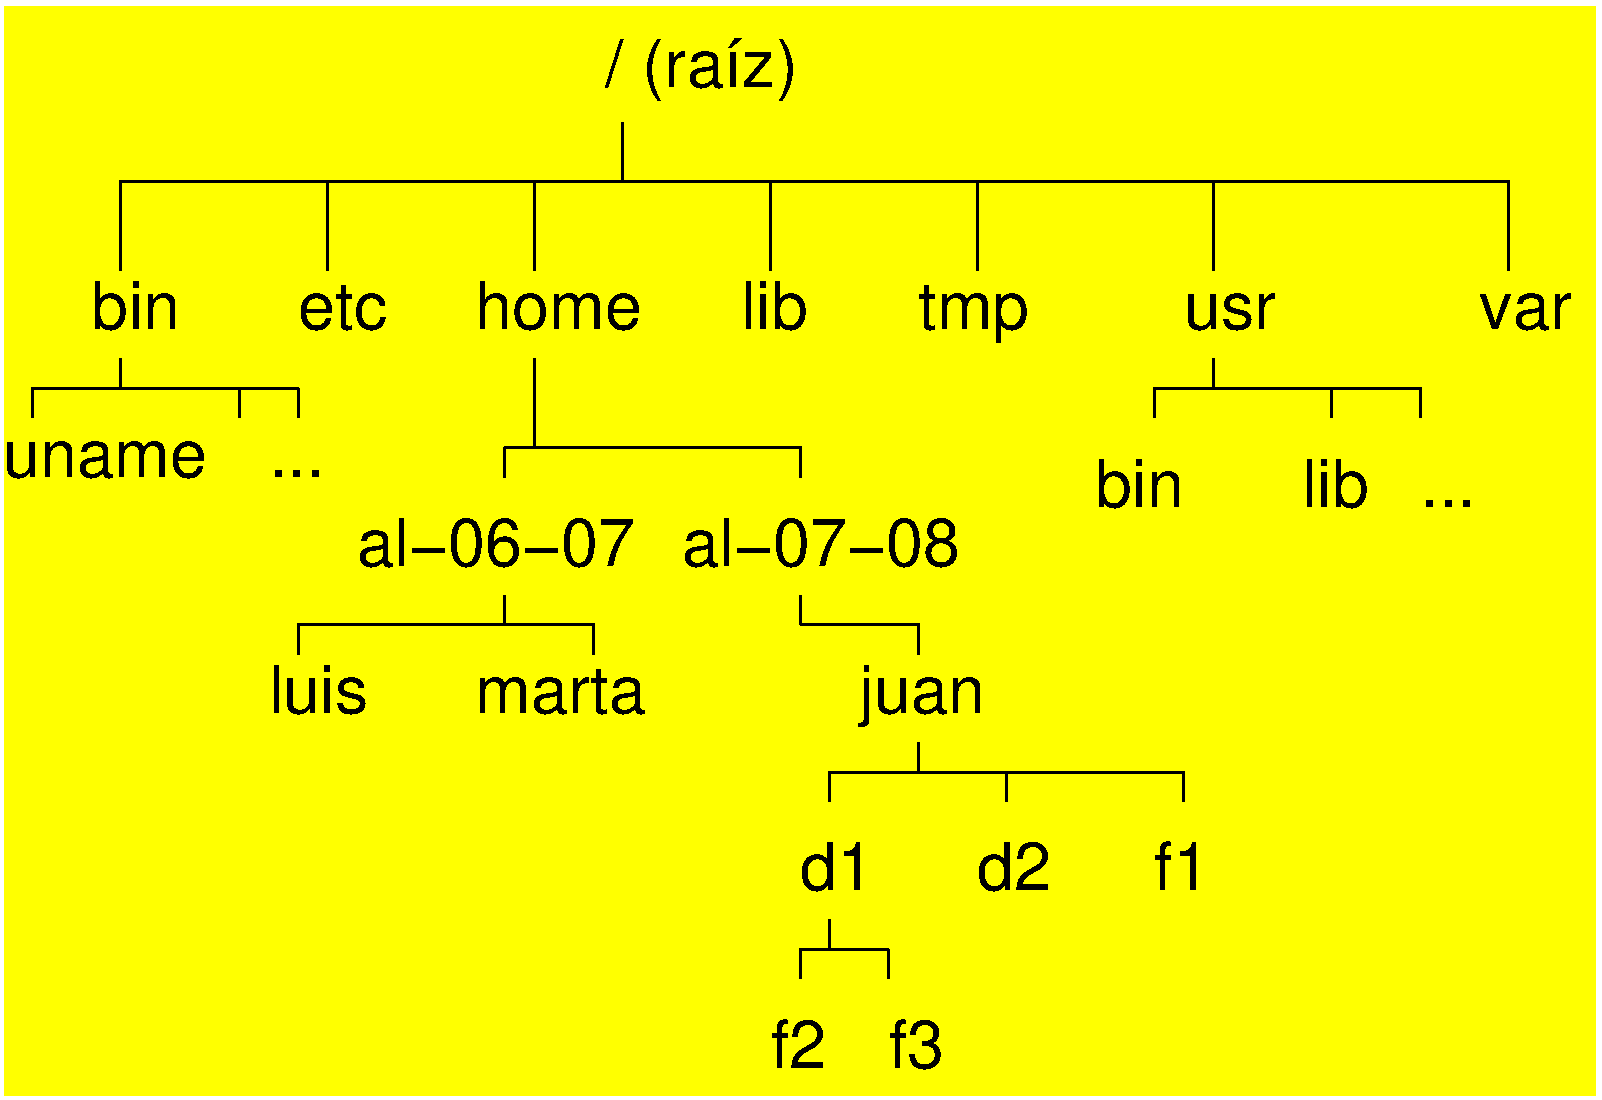
\includegraphics[width=5cm]{figs/unix-tree-2}
  \end{minipage}
  \begin{minipage}{5.5cm}
  \begin{itemize}
  \item Ejemplos:
    \begin{footnotesize}
      \begin{itemize}
      \item Trayecto absoluto de \verb|f2|:
\begin{verbatim}
/home/al-07-08/juan/d1/f2
\end{verbatim}
      \item Trayecto relativo de \verb|f2| si el directorio de trabajo es \verb|juan|:
\begin{verbatim}
d1/f2
\end{verbatim}
      \item Trayecto relativo de \verb|f2| si el directorio de trabajo es \verb|d2|:
\begin{verbatim}
../d1/f2
\end{verbatim}
      \item Trayecto relativo de \verb|var| si el directorio de trabajo es \verb|luis|:
\begin{verbatim}
../../../var
\end{verbatim}



      \end{itemize}
    \end{footnotesize}    
  \end{itemize}
  \end{minipage}


\end{frame}



%%---------------------------------------------------------------

%%---------------------------------------------------------------
\begin{frame}[fragile]


  \begin{itemize}
  \item cd: Cambia el directorio de trabajo (\emph{change directory})
    \begin{footnotesize}
      \begin{tabbing}
        \verb|echo |\hspace{1cm} \= No escribe nada útil aquí\kill
        \verb|cd d1| \> Cambia desde el directorio de trabajo actual a su
        subdirectorio \verb|d1|\\
        \verb|cd /home| \> Cambia desde cualquier directorio al
        directorio \verb|/home|\\
        \verb|cd ..| \> Cambia desde el directorio de trabajo actual a su
        directorio padre\\ \> (sube un directorio)\\
        \verb|cd| \> Cambia al directorio por defecto (hogar) del usuario
      \end{tabbing}
    \end{footnotesize}
    
  \item ls: Muestra los contenidos de un directorio (\emph{list})
    \begin{footnotesize}
      \begin{tabbing}
        \verb|echo |\hspace{1cm} \= No escribe nada útil aquí\kill
        \verb|ls| \> Muestra el contenido del directorio de trabajo \\
        \verb|ls d1| \> Muestra el contenido del subdirectorio \verb|d1|\\
        \verb|ls /home| \> Muestra el contenido de \verb|/home|\\
      \end{tabbing}
    \end{footnotesize}


  \end{itemize}


\end{frame}


%%---------------------------------------------------------------
\section{Operaciones básicas con ficheros y directorios}
%%---------------------------------------------------------------

\begin{frame}[fragile]
\frametitle{touch}
Cambia la fecha a un fichero, o lo crea si no existe

\verb|touch <fichero>|
\begin{itemize}
\item
Si
\verb|<fichero>|
existe, le pone la fecha actual
\item
Si
\verb|<fichero>|
no existe, crea un fichero vacío con este nombre
\end{itemize}

\verb|touch -d <fecha/hora>  <fichero>|

Modifica la fecha de último acceso al fichero

  \begin{footnotesize}
  \begin{verbatim}
touch -d 2007-02-28 fichero      # cambia la fecha
touch -d 15:41 fichero           # cambia la fecha
  \end{verbatim}
  \end{footnotesize}


\end{frame}

%%---------------------------------------------------------------
\begin{frame}[fragile]
\frametitle{mkdir: Creación de directorios}

   mkdir: Crea directorios (\emph{make directory})

\verb|mkdir <fichero>|
\begin{itemize}
\item
\verb|mkdir d3|  

Crea d3 como subdirectorio del directorio actual

\item
\verb|mkdir d4 d5|  

Crea d4 y d5 como subdirectorios del directorio de trabajo actual

\item
\verb|mkdir /tmp/ppp|  

Crea el directorio \verb|/tmp/ppp| 

\item
\verb|mkdir -p d6/d7|  

Crea debajo de directorio de trabajo \verb|d6| (si no existe), y crea \verb|d7| debajo de \verb|d6|

\end{itemize}

%  \item rmdir: Borra directorios \textbf{vacíos} (\emph{remove directory})
%    \begin{footnotesize}
%      \begin{tabbing}
%        \verb|echo hola|\hspace{1cm} \= No escribe nada útil aquí\kill
%        \verb|rmdir d3| \> Borra d3 (si está vacío)\\
%        \verb|rmdir d4 d5| \> Borra d4 y d5 (vacíos)\\
%        \verb|rmdir /tmp/ppp| \> Borra el directorio \verb|/tmp/ppp| (vacío)\\
%        \verb|rmdir -p d6/d7| \> Borra \verb|d6/d7| (vacío) y luego
%        borra \verb|d6|, subdirectorio del directorio actual\\
%      \end{tabbing}
%    \end{footnotesize}


\end{frame}

%%---------------------------------------------------------------

%%---------------------------------------------------------------
\begin{frame}[fragile]
\frametitle{Copiar, mover y renombrar}

\begin{itemize}
\item
La órden \verb|cp| copia ficheros
\item
La órden \verb|mv| mueve y renombra ficheros
\end{itemize}

En primer lugar mostraremos el uso básico, después
las opciones completas


\res{Copiar un fichero:}

tengo 
  \begin{footnotesize}
  \begin{verbatim}
/tmp/probando/quijote.txt
  \end{verbatim}
  \end{footnotesize}

quiero 
  \begin{footnotesize}
  \begin{verbatim}
/tmp/probando/quijote.txt
/tmp/probando/quijote_repetido.txt
  \end{verbatim}
  \end{footnotesize}

hago
  \begin{footnotesize}
  \begin{verbatim}
cd /tmp/probando
cp quijote.txt quijote_repetido.txt
  \end{verbatim}
  \end{footnotesize}

\end{frame}
%%----------------------------------------------
\begin{frame}[fragile]

\res{Renombrar un fichero:}

tengo 
  \begin{footnotesize}
  \begin{verbatim}
/tmp/probando/quijote.txt
  \end{verbatim}
  \end{footnotesize}
quiero 
  \begin{footnotesize}
  \begin{verbatim}
/tmp/probando/don_quijote.txt
  \end{verbatim}
  \end{footnotesize}

hago
  \begin{footnotesize}
  \begin{verbatim}
cd /tmp/probando
mv quijote.txt don_quijote.txt
  \end{verbatim}
  \end{footnotesize}


\end{frame}
%%----------------------------------------------
\begin{frame}[fragile]

\res{Copiar un fichero en un directorio distinto}

  \begin{footnotesize}
  \begin{verbatim}
tengo
/tmp/probando/quijote.txt
  \end{verbatim}
  \end{footnotesize}
quiero
  \begin{footnotesize}
  \begin{verbatim}
/tmp/probando/quijote.txt
/tmp/otro_probando/quijote.txt
  \end{verbatim}
  \end{footnotesize}

voy al directorio destino
  \begin{footnotesize}
  \begin{verbatim}
cd /tmp/otro_probando/
  \end{verbatim}
  \end{footnotesize}

  \begin{footnotesize}
  \begin{verbatim}
#copio     "el fichero"         "aquí"
cp    /tmp/probando/quijote.txt    .  
  \end{verbatim}
  \end{footnotesize}

\end{frame}
%%----------------------------------------------
\begin{frame}[fragile]

\res{Mover un fichero a un directorio distinto}

tengo
  \begin{footnotesize}
  \begin{verbatim}
/tmp/probando/quijote.txt
  \end{verbatim}
  \end{footnotesize}
quiero
  \begin{footnotesize}
  \begin{verbatim}
/tmp/otro_probando/quijote.txt
  \end{verbatim}
  \end{footnotesize}


voy al destino
  \begin{footnotesize}
  \begin{verbatim}
cd /tmp/otro_probando/
  \end{verbatim}
  \end{footnotesize}

  \begin{footnotesize}
  \begin{verbatim}
# muevo "el fichero"        "aquí"
mv /tmp/probando/quijote.txt   .  
  \end{verbatim}
  \end{footnotesize}

\end{frame}


%%---------------------------------------------------------------

\begin{frame}[fragile]
\frametitle{cp: Copiar 1 fichero ordinario }
      \verb|cp <origen> <destino>|

cp (\emph{copy}) con dos argumentos.  \verb| <origen>| es un fichero ordinario

  \begin{itemize}
    \item Si el segundo argumento es un directorio

        Hace una copia del fichero \verb|<origen>| dentro del directorio \verb|<destino>| 


    \item Si el segundo argumento NO es un directorio (es un fichero o no existe nada con ese nombre)

        Hace una copia del fichero \verb|<origen>| y le pone como nombre \verb|<destino>| 
  \end{itemize}

Como siempre, tanto 
\verb|<origen>|
como
\verb|<destino>|
pueden indicarse con trayecto relativo o con trayecto absoluto


Ejemplos:

  \begin{footnotesize}
  \begin{verbatim}
cp holamundo.py /tmp
cp ~/prueba.txt .
cp /home/jperez/prueba.txt prueba2.txt
  \end{verbatim}
  \end{footnotesize}

\end{frame}



%%---------------------------------------------------------------


\begin{frame}[fragile]
\frametitle{cp: Copiar 1 directorio }
  
      \verb|cp -r <origen> <destino>|

Si \verb|<origen>|
es un directorio, es necesario añadir la opción \verb|-r| (\emph{recursive})


\begin{itemize}
\item
Si \verb|<destino>| es un fichero ordinario, se produce un error
\item
Si \verb|<destino>| es un directorio, el directorio \verb|<origen>| se copia dentro
\item
Si \verb|<destino>| no existe, se le pone ese nombre a la copia 
\end{itemize}

Ejemplos
  \begin{footnotesize}
  \begin{verbatim}
cp -r ~  /tmp
cp -r /var/tmp/aa .
cp -r ~  /tmp/copia_de_mi_home
  \end{verbatim}
  \end{footnotesize}

\end{frame}


%%---------------------------------------------------------------
\begin{frame}[fragile]
\frametitle{cp: Copiar varios  ficheros ordinarios }
      \verb|cp <origen1> <origen2> .... <destino>|

cp (\emph{copy}) con varios argumentos.  
Los ficheros 
      \verb|<origen1> <origen2> ....|
se copian en el directorio
      \verb| <destino>|

  \begin{itemize}
    \item 
        \verb|<destino>| tiene que ser un directorio (o se producirá un error)
     \item
        \verb|<origen1>, <origen2>,...| tienen que ser ficheros ordinarios (o un mensaje indicará que no se están copiando) 
     
  \end{itemize}



Ejemplos:

  \begin{footnotesize}
  \begin{verbatim}
cp holamundo.py /home/jperez/prueba1.txt ../prueba2.txt /tmp
cp bin/*.py /tmp
  \end{verbatim}
  \end{footnotesize}

\end{frame}



%%---------------------------------------------------------------
\begin{frame}[fragile]
\frametitle{cp: Copiar varios  ficheros o directorios }
      \verb|cp -r <origen1> <origen2> .... <destino>|

Este caso es idéntico al anterior, solo que si 
      \verb|<origen1>|
o
      \verb|<origen2>|
o
 \verb|...|
son directorios, es necesaria la opción \verb|-r|



Ejemplos:

  \begin{footnotesize}
  \begin{verbatim}
cp -r holamundo.py /home/jperez /tmp
  \end{verbatim}
  \end{footnotesize}

\end{frame}



%%---------------------------------------------------------------

\begin{frame}[fragile]
\frametitle{mv: mover o renombrar ficheros y directorios }
      \verb|mv <origen> <destino>|

Mover dentro del mismo directorio equivale a renombrar

%mv (\emph{mv}) con dos argumentos  
\verb| <origen>| es un fichero o un directorio

  \begin{itemize}
    \item Si el segundo argumento es un directorio

        Mueve \verb|<origen>| dentro del directorio \verb|<destino>| 


    \item Si el segundo argumento no existe 

        Mueve \verb|<origen>| a  \verb|<destino>| 


     \item Si \verb|<destino>| es un fichero
  \begin{itemize}
\item
y  \verb|<origen>| es un fichero, \verb|<origen>| pasa a llamarse
\verb|<destino>|
y el anterior
\verb|<destino>|
despararece
\item
y el primero es un directorio, se produce un error
  \end{itemize}


  \end{itemize}

%Como siempre, tanto 
%\verb|<origen>|
%como
%\verb|<destino>|
%pueden indicarse con trayecto relativo o con trayecto absoluto


Ejemplos:

  \begin{footnotesize}
  \begin{verbatim}
mv holamundo.py /tmp
mv ~/prueba.txt .
mv /home/jperez/prueba.txt prueba2.txt
  \end{verbatim}
  \end{footnotesize}

\end{frame}



%%---------------------------------------------------------------
\begin{frame}[fragile]

mv con más de dos argumentos

\verb|mv <origen1> <origen2> ...  <destino>|

\verb|<destino>|  debe ser un directorio existente

%mv (\emph{mv}) con dos argumentos  
\verb|<origen1>, <origen2>...| pueden ser ficheros ordinarios o directorios


Ejemplos:
  \begin{footnotesize}
  \begin{verbatim}
mv holamundo.py /home/jperez/prueba1.txt ../prueba2.txt /tmp
mv *.txt texto
  \end{verbatim}
  \end{footnotesize}


\end{frame}



%%---------------------------------------------------------------

%\begin{frame}[fragile]
%
%  \begin{itemize}
%  \item cp: Copia ficheros (\emph{copy})\\
%    \vspace{-2mm}\\\textbf{VARIANTE 2}: \verb|cp <origen1> <origen2> ... <destino>|
%    \begin{footnotesize}
%      \begin{tabbing}
%        a\hspace{4mm} \= No escribe nada útil aquí\kill
%        \>\verb|<origen1>|, \verb|<origen2>| \ldots son los ficheros
%        origen de la copia\\ 
%        \> \verb|<destino>| es el directorio en el que se guardará la
%        copia de los ficheros \verb|<origen>|\\
%        \> Si se añade la opción \verb|-r| uno o más de los \verb|<origen>| puede ser
%        un directorio, \\ \> y en ese caso sus contenidos se copian
%        recursivamente en \verb|<destino>|
%      \end{tabbing}
%    \end{footnotesize}
%
%    \begin{footnotesize}
%      \begin{tabbing}
%        \verb|echo hola|\hspace{25mm} \= No escribe nada útil aquí\kill
%        \verb|cp f1 f2 f3 d1| \> Copia \verb|f1|, \verb|f2| y
%        \verb|f3| con el mismo nombre al subdirectorio\\\> de DT \verb|d1|\\
%        \verb|cp /tmp/f1 /tmp/f2 .| \> Copia \verb|/tmp/f1| y
%        \verb|/tmp/f2| al DT, con el mismo nombre\\
%        \verb|cp -r d1 d2 d3| \> Copia \verb|d1| y todos sus
%        contenidos, y \verb|d2| y todos sus\\ 
%        \> contenidos al subdirectorio de DT \verb|d3|\\
%      \end{tabbing}
%    \end{footnotesize}
%  \end{itemize}
%
%\end{frame}
%
%%%---------------------------------------------------------------
%
%
%\begin{frame}[fragile]
%
%  \begin{itemize}
%  \item mv: Mueve (y/o renombra) ficheros (\emph{move})\\
%    \vspace{-2mm}\\\textbf{VARIANTE 1}: \verb|mv <origen> <destino>|
%    \begin{footnotesize}
%      \begin{tabbing}
%        a\hspace{4mm} \= No escribe nada útil aquí\kill
%        \>\verb|<origen>| es el origen de la copia\\\
%        \> Si \verb|<destino>| es un directorio, es el lugar al que se moverá
%        el \verb|<origen>|\\
%        \>Si \verb|<destino>| no es un directorio, es el nuevo nombre
%        para el \verb|<origen>|\\
%        \>Si \verb|<origen>| y \verb|<destino>| están en el mismo
%        directorio, este mandato simplemente\\\> renombra.
%      \end{tabbing}
%    \end{footnotesize}
%
%    \begin{footnotesize}
%      \begin{tabbing}
%        \verb|echo hola|\hspace{1cm} \= No escribe nada útil aquí\kill
%        \verb|mv f1 f2| \> Cambia el nombre de \verb|f1| al nombre \verb|f2|, en DT \\
%        \verb|mv f1 d1| \> Mueve \verb|f1| con el mismo nombre al subdirectorio de DT
%        \verb|d1|\\
%      \end{tabbing}
%    \end{footnotesize}
%  \end{itemize}
%
%\end{frame}
%
%%%---------------------------------------------------------------
%
%
%\begin{frame}[fragile]
%
%  \begin{itemize}
%  \item mv: Mueve (y/o renombra) ficheros (\emph{move})\\
%    \vspace{-2mm}\\\textbf{VARIANTE 2}: \verb|mv <origen1> <origen2> ... <destino>|
%    \begin{footnotesize}
%      \begin{tabbing}
%        a\hspace{4mm} \= No escribe nada útil aquí\kill
%        \>\verb|<origen1>|, \verb|<origen2>| \ldots son los ficheros o
%        directorios que se mueven\\ 
%        \> \verb|<destino>| es el directorio al que se moverán los \verb|<origen>|\\
%      \end{tabbing}
%    \end{footnotesize}
%
%    \begin{footnotesize}
%      \begin{tabbing}
%        \verb|echo hola|\hspace{1cm} \= No escribe nada útil aquí\kill
%        \verb|mv f1 f2 f3 d1| \> Mueve \verb|f1|, \verb|f2| y
%        \verb|f3| con el mismo nombre al subdirectorio de DT \verb|d1|\\
%      \end{tabbing}
%    \end{footnotesize}
%  \end{itemize}
%
%\end{frame}
%
%
%%%---------------------------------------------------------------
%
%
%\begin{frame}[fragile]
%
%  \begin{itemize}
%  \item rm: Borra un fichero (\emph{remove}):
%
%    \verb|rm <elemento1> <elemento2> ... |
%    \begin{footnotesize}
%      \begin{tabbing}
%        a\hspace{4mm} \= No escribe nada útil aquí\kill
%        \>\verb|<elemento1>|, \verb|<elemento2>| \ldots son los ficheros
%        que se borrarán\\ 
%        \> Si se añade la opción \verb|-r| uno o más de los \verb|<elemento>s| puede ser
%        un directorio, \\ \> y en ese caso todos sus contenidos se
%        borran recursivamente (\textbf{puede ser peligroso})
%      \end{tabbing}
%    \end{footnotesize}
%
%    \begin{footnotesize}
%      \begin{tabbing}
%        \verb|echo hola|\hspace{1cm} \= No escribe nada útil aquí\kill
%        \verb|rm f1| \> Borra el fichero \verb|f1| del DT\\
%        \verb|rm f1 f2 f3| \> Borra los ficheros \verb|f1|,
%        \verb|f2| y \verb|f3| del DT\\
%        \verb|rm -r d1| \> Borra el directorio \verb|d1| del DT,
%        \textbf{y todos sus contenidos}\\
%      \end{tabbing}
%    \end{footnotesize}
%  \end{itemize}
%
%\end{frame}
%
%
%

%%---------------------------------------------------------------

\begin{frame}[fragile]
\frametitle{Tipos de fichero}
\begin{itemize} 
\item Tradicionalmente en Unix los ficheros no llevaban extensión\\
No hay un programa asociado a cada extension\\
\verb|    file mifichero          |   \\  
Indica el tipo del fichero. No importa si 
tiene extensión, si no la tiene, o si es errónea
%\item
%el shell nos ayuda con \emph{autocompletar} (tab)\\
%y \emph{history} (cursor arriba) 
%\item ls, pwd, cd
%\item 
%\verb|cp|  \emph{origen} \emph{destino} 
%
%\verb|cp -r  /tmp  .|\\Copia el directorio \verb|tmp| al directorio actual 
%
%\verb|cp  /tmp/*  .|\\Copia los ficheros del directorio \verb|tmp| al directorio actual \\
%\verb|cp  -r  /usr/share/ejemplo  ~/pruebas|\\Copia el directorio \verb|ejemplo| en el directorio \verb|pruebas| del \emph{home} del usuario actual.

%\item 
%\verb|mv| \emph{origen} \emph{destino}\\Mueve un fichero. Equivale a renombrar
%
%\verb|cp| y
%\verb|mv| pueden recibir más de 2 argumentos. 
%
%En ese caso, el último debe ser un directorio
\end{itemize}

Supongamos que tenemos un fichero y no sabemos
con qué programa podemos
abrirlo. P.e. desconocemos que tenemos
instalado evince para abrir ficheros pdf


\begin{itemize}
\item
En Linux

\begin{itemize}
\item
Si nuestro escritorio es gnome, podemos ejecutar

\verb|gnome-open  fichero.extension| 

\item
	Si usamos KDE, 
\verb|kde-open fichero.extension| 
\item
	Para gnome, KDE y muchos otros
\verb|xdg-open fichero.extension| 
		 
\end{itemize}

\item
	En Mac OS

\verb|open  fichero.extension| 

\end{itemize}


\end{frame}

%%-----------------------------

\begin{frame}[fragile]
\frametitle{Borrado de un fichero}
\begin{itemize} 

\item 
\verb|rm| \emph{fichero} \\borra fichero  \footnote{Cuando hablemos de enlaces veremos una definición más exacta} \\
\verb|rm  -r| \emph{directorio} 

Borra un directorio y todo su contenido
%\item 
%\verb|mkdir|
%
%Crea un directorio

\end{itemize}
\end{frame}

%%---------------------------------------------------------------
\begin{frame}[fragile]
%\section{}
Un usuario de MS-DOS podría intentar hacer

\verb| mv *.txt *.doc   # ¡MAL!  No funciona, y puede ser fatal|

Supongamos que tenemos en el directorio actual
\begin{footnotesize}
\begin{verbatim}
carta1.txt 
carta2.doc
\end{verbatim}
\end{footnotesize}
Tras expandir los asteriscos, el resultado es

\verb|mv carta1.txt carta2.doc  # destruimos el segundo fichero!|


Una solución posible \footnote{Siempre que solo haya un punto en el nombre}:
\begin{footnotesize}
\begin{verbatim}
#!/bin/bash
for fichero in *.txt
do
    nombre=$(echo $fichero | cut -d. -f1)
    extension=$(echo $fichero | cut -d. -f2)
    mv $fichero $nombre.doc
done
\end{verbatim}
\end{footnotesize}



\end{frame}



%%---------------------------------------------------------------
\section{Enlaces}
%%---------------------------------------------------------------
\begin{frame}[fragile]
\frametitle{Enlace duro}
Un nuevo nombre para el fichero\\
 \verb|ln a b|   
\begin{itemize} 
\item
Ambos nombres deben pertenecer al mismo sistema de ficheros 

\item
Pueden ser útiles para mantener los ficheros ordenados y  \emph{a mano}, además
de  para evitar algunos
borrados accidentales
\item

Dado un fichero, se sabe cuántos nombres tiene. Para saber cuáles son sus nombres, habría que buscarlos

\item
La mayoría de los S.O. no permiten enlaces duros a directorios, puesto que
podría provocar bucles difíciles de detectar
% Leopard sí lo permite

%\item mount
%\item /etc/fstab
%\item nfs
\end{itemize}
\verb|rm| borra un nombre de un fichero\\
si es el último, borra el fichero.\\

\end{frame}


%%---------------------------------------------------------------
\begin{frame}[fragile]
\begin{figure}
\centerline{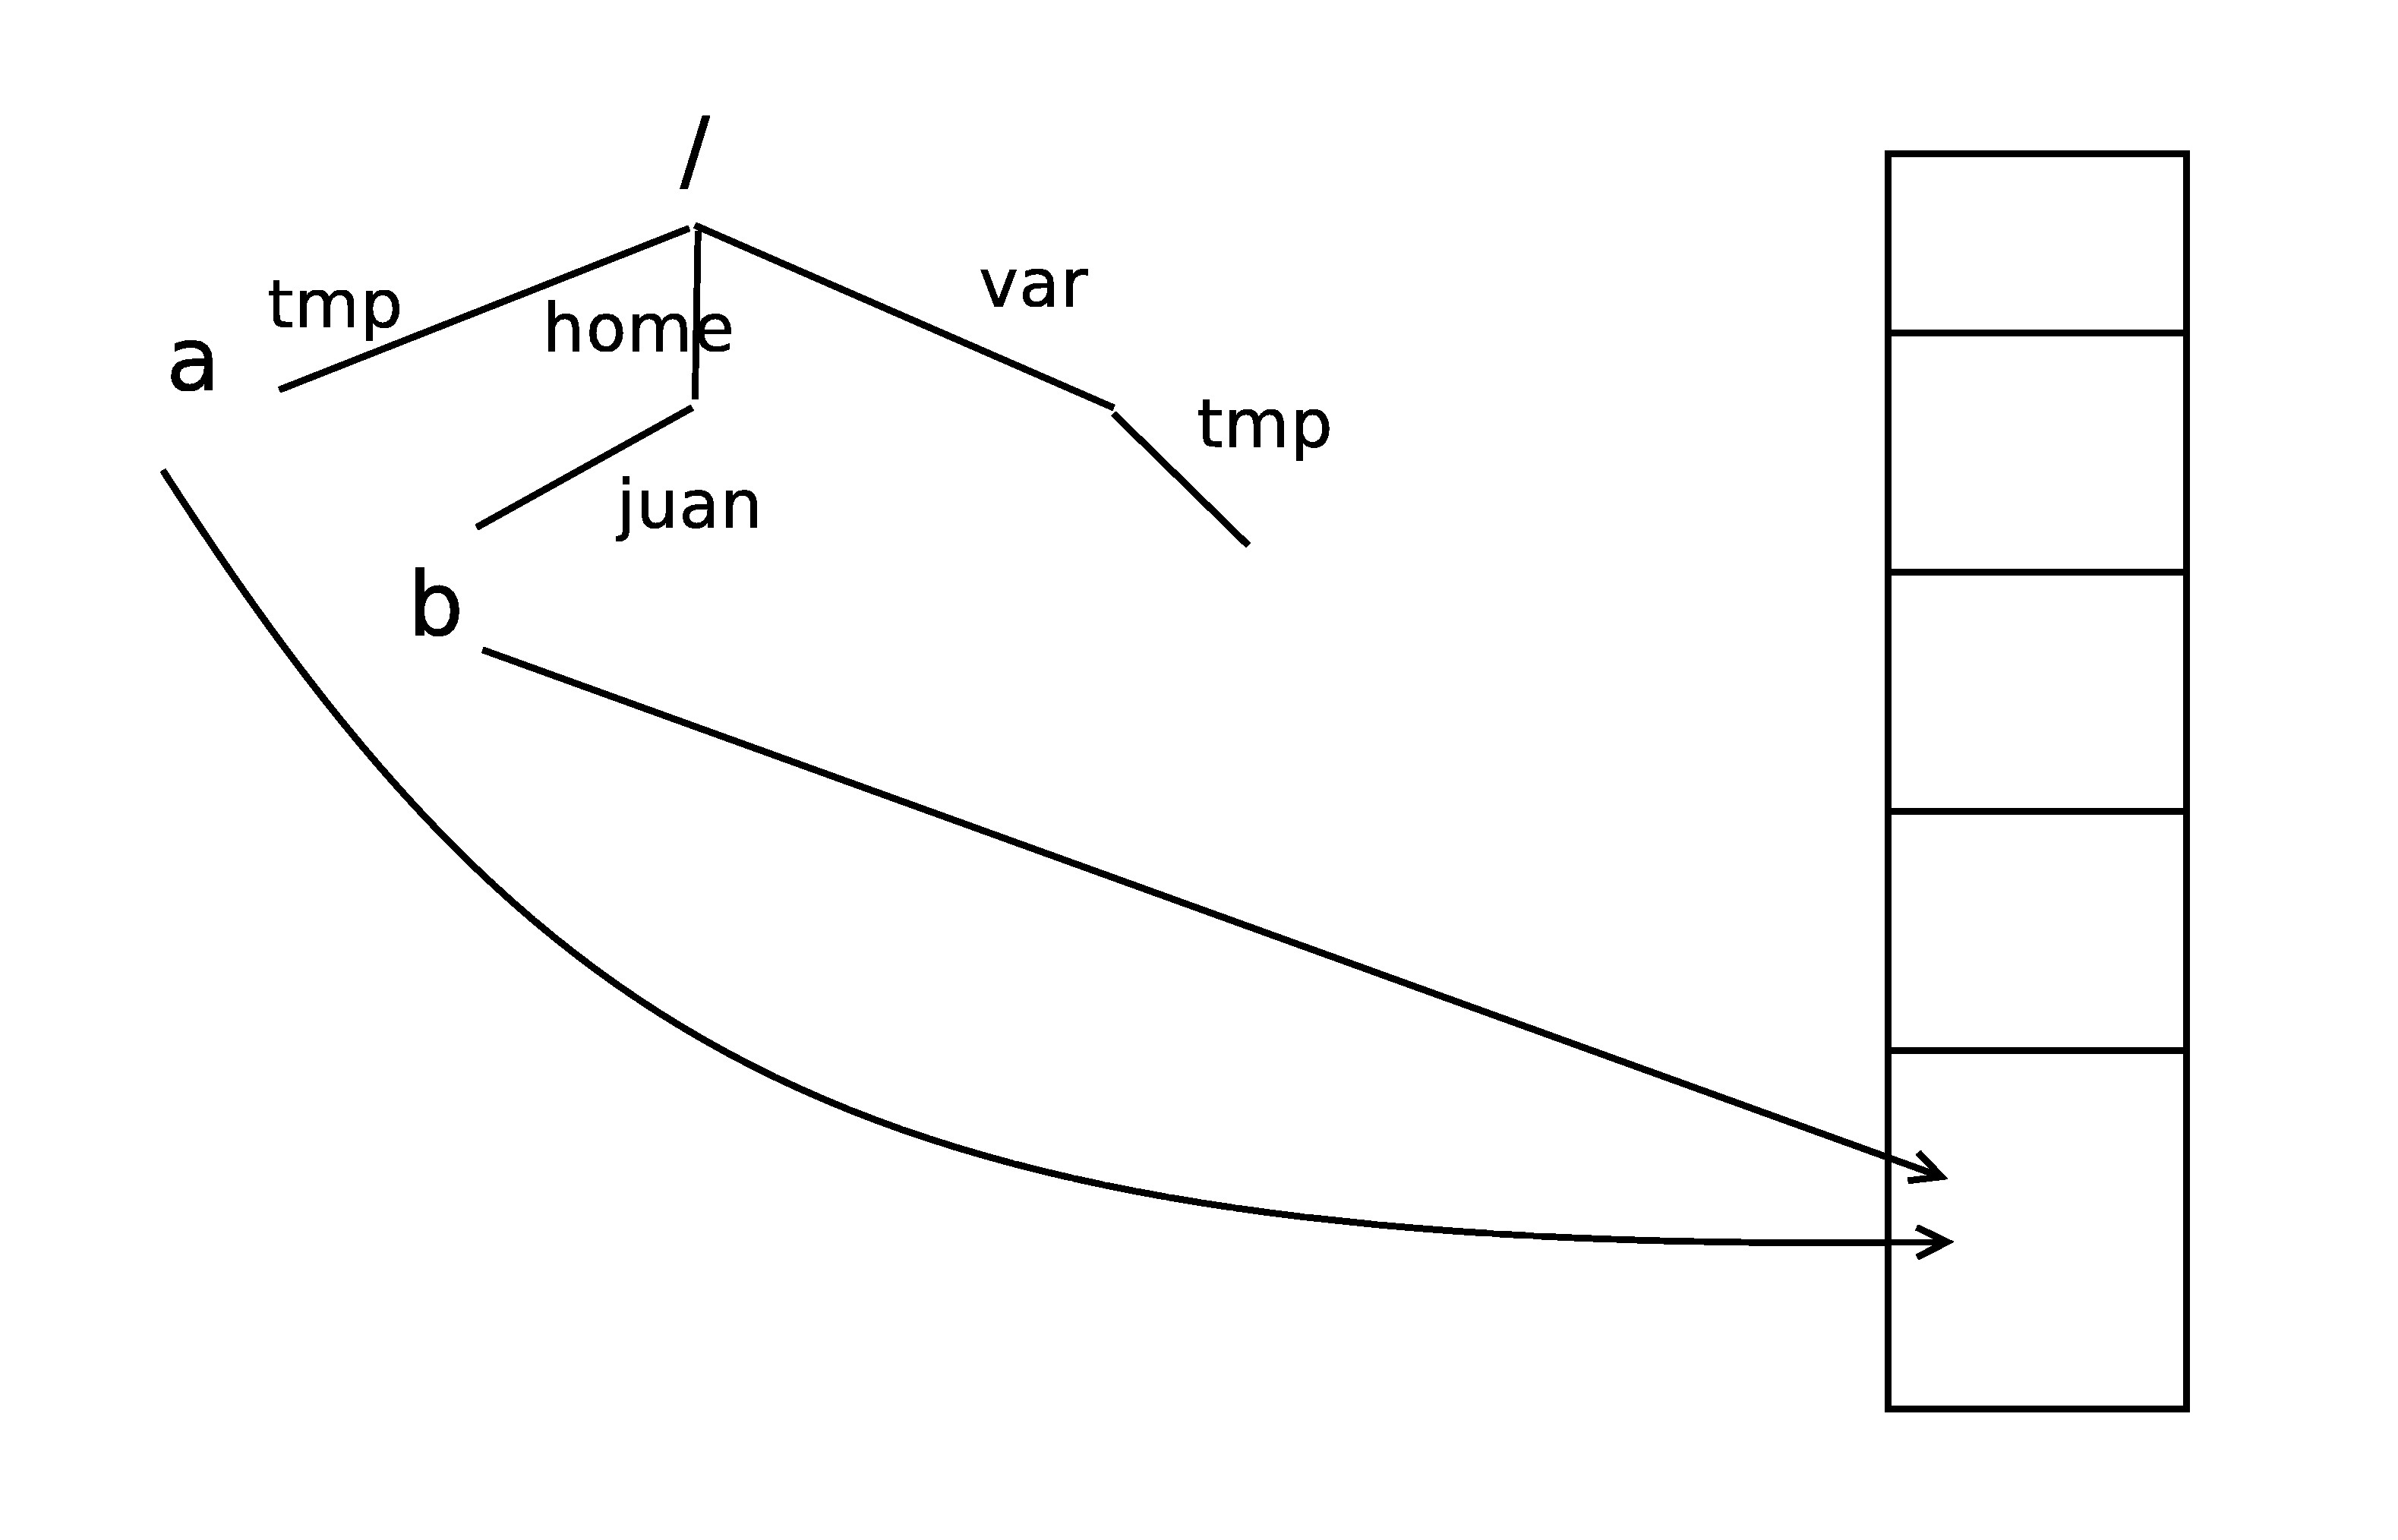
\includegraphics[width=8cm]{figs/enlace_duro}}
\caption{Enlace Duro}
\end{figure}
\end{frame}



%%---------------------------------------------------------------
\begin{frame}[fragile]
\frametitle{Enlace blando o simbólico}

Un nuevo fichero que apunta a un nombre\\
 \verb|ln -s /home/juan/b c|   
\begin{itemize}	
\item
Sirven principalmente para mantener ficheros ordenados y \emph{a mano}

\item 
Puede hacerse entre distintos sistemas de ficheros
\item
Puede enlazarse un directorio
\item 
Con enlaces simbólicos, si se borra el original\\
el enlace queda roto
\item 
Puede ser conveniente indicar el fichero original con
el path completo, así, si lo movemos sigue apuntando al mismo sitio.

En otras ocasiones es imprescindible indicar el
fichero original con path completo
% Miguel, febrero 2010. Creo antiguamente era obligatorio si
% invocabas el enlace desde un directorio distinto: si
% lo definias relativo y lo invocabas desde un lugar distinto,
% el enlace se consideraba desde el lugar donde invocas, no
% desde donde estaba creado. Pero no estoy seguro
\end{itemize}


\end{frame}




%%---------------------------------------------------------------
\begin{frame}[fragile]
\begin{figure}
\centerline{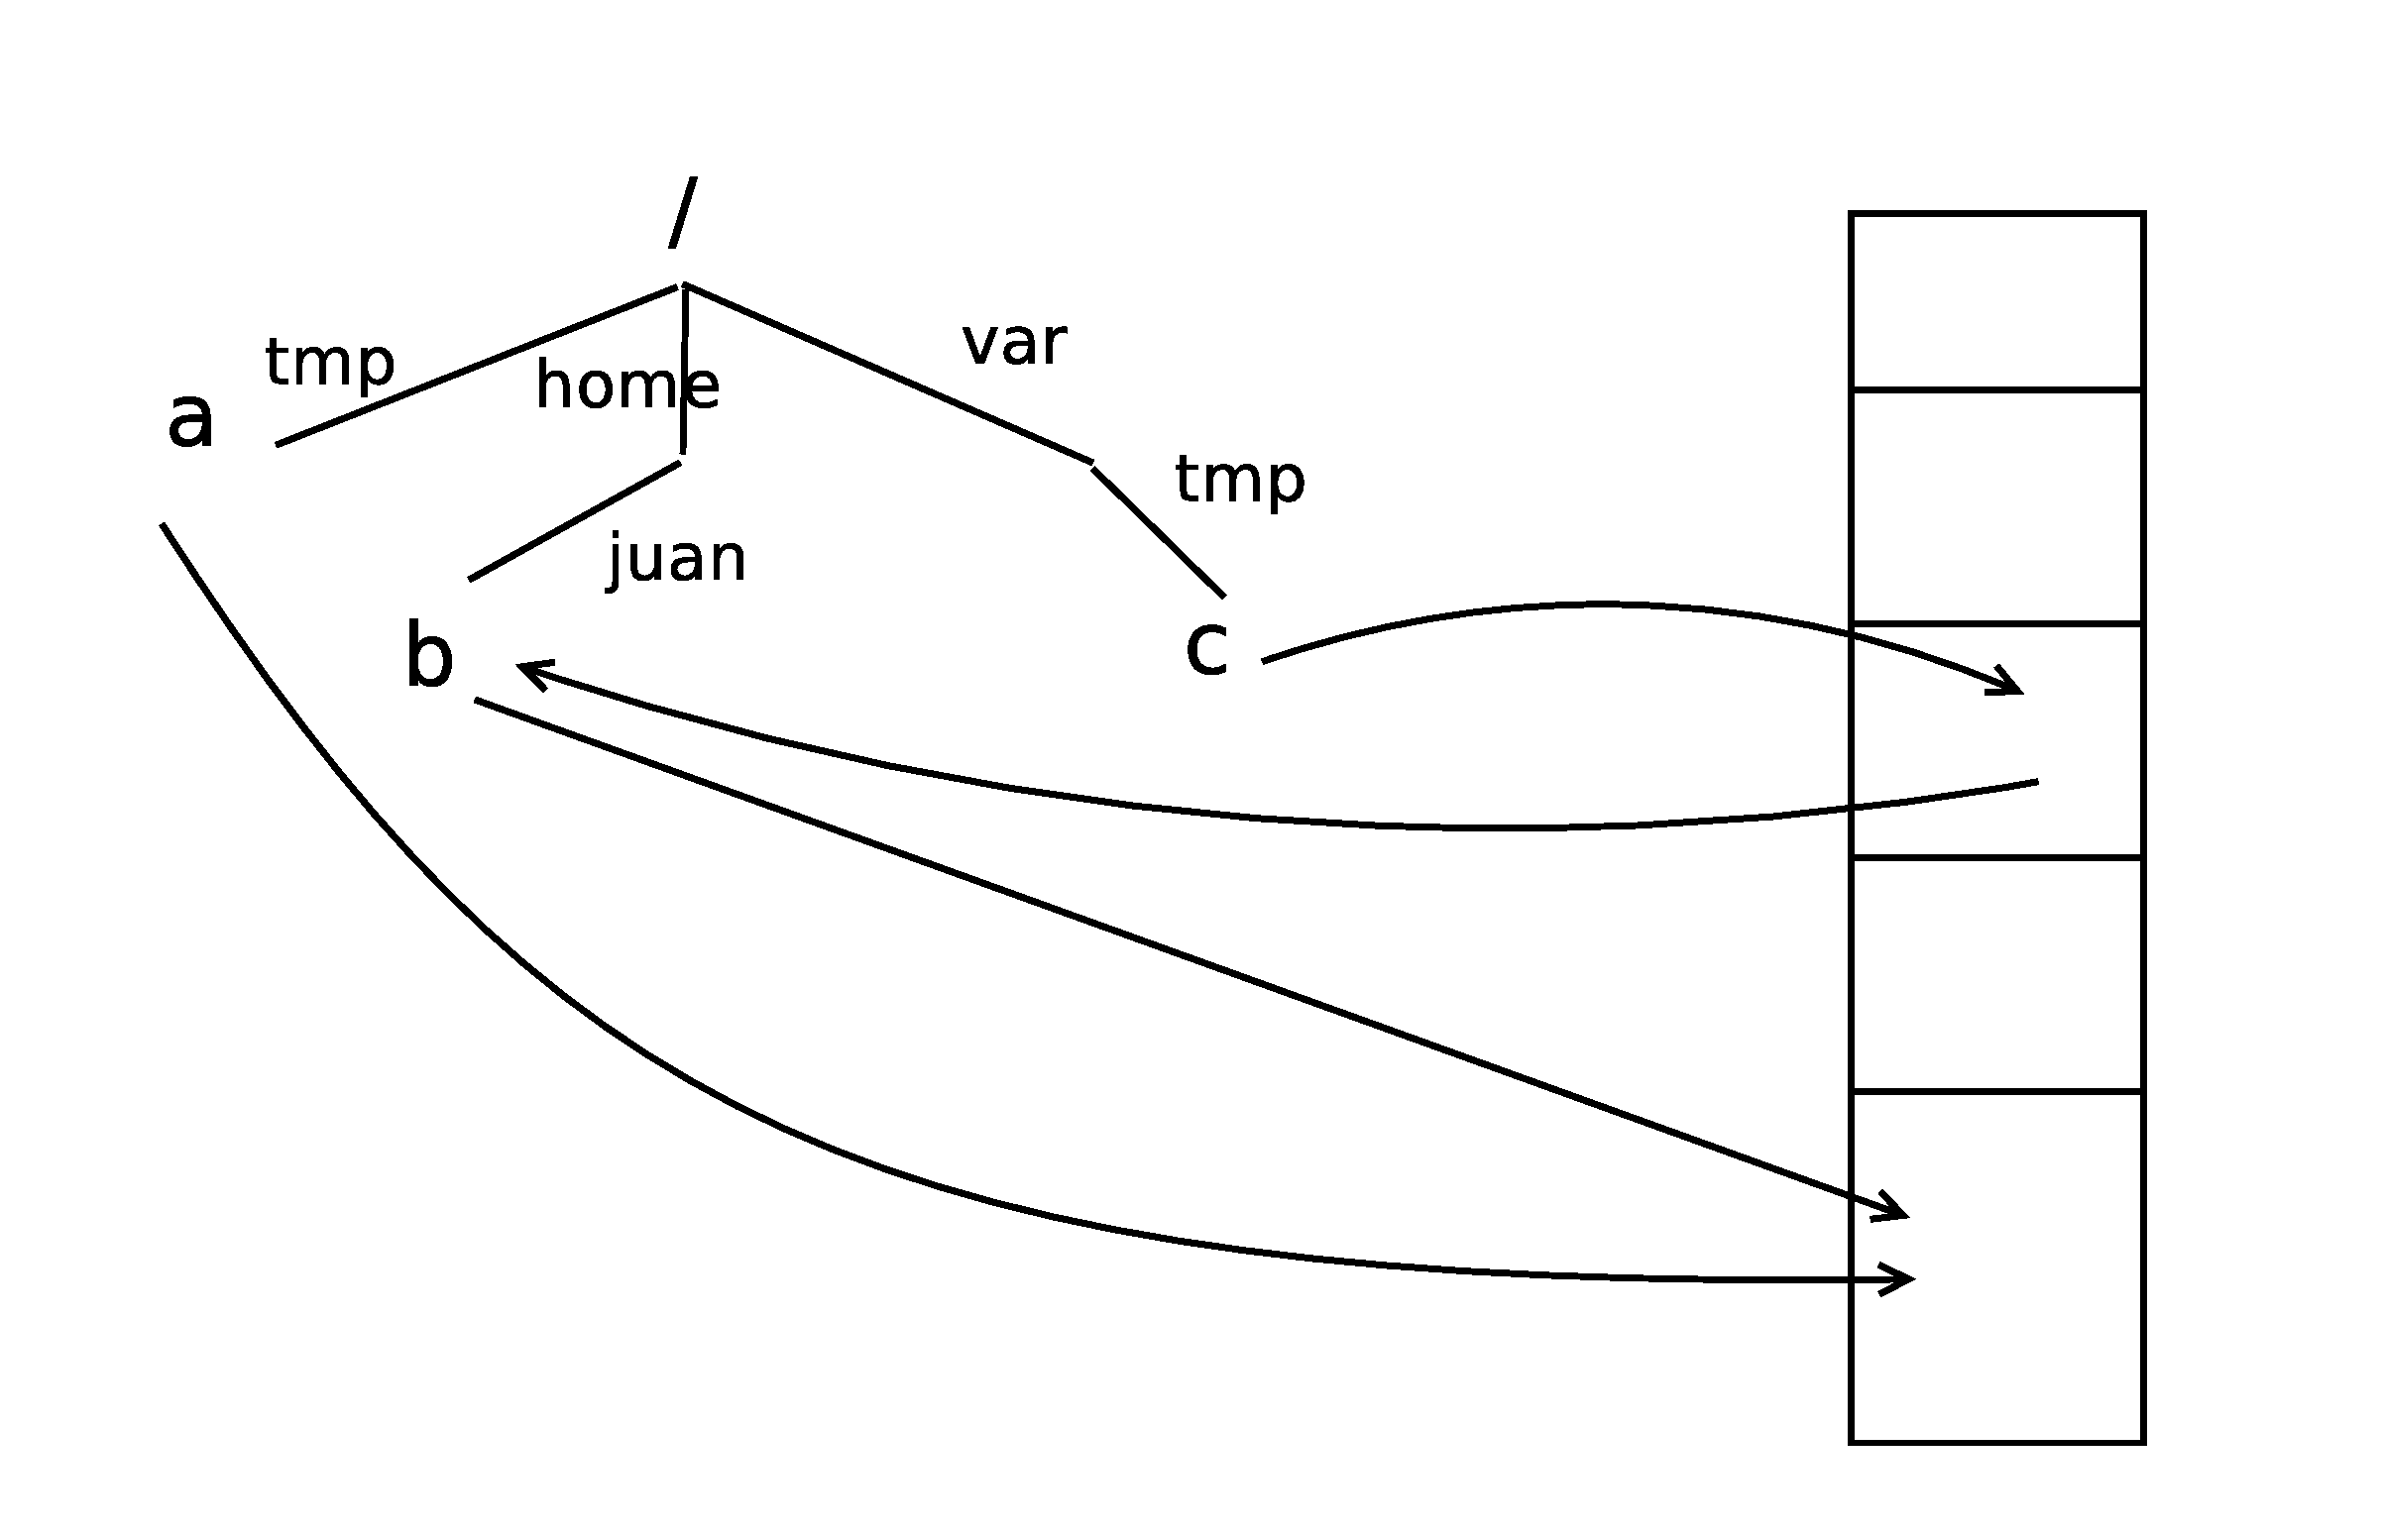
\includegraphics[width=8cm]{figs/enlace_blando}}
\caption{Enlace Simbólico}
\end{figure}
\end{frame}


%%---------------------------------------------------------------
%\begin{frame}[fragile]
%\section{Background}
%\begin{itemize}        
%\item background
%\item \texttt{acroread file.1 \&}
%\item jobs
%\item bg, fg
%\end{itemize}
%\end{frame}

%%---------------------------------------------------------------
  \section{Mandatos de uso básico de la red}
%%---------------------------------------------------------------



%\begin{frame}[fragile]
%  \begin{itemize}
%  \item \res{hostname}: Muestra el nombre de la máquina
%    \begin{footnotesize}
%      \begin{tabbing}
%        \verb|echo hola|\hspace{2.5cm} \= No escribe nada útil aquí\kill
%        \verb|hostname| \>  Muestra el nombre de la máquina \\
%        \verb|hostname -d| \>  Muestra el dominio de DNS de la máquina \\
%        \verb|hostname -i| \>  Muestra la dirección IP de la máquina \\
%        \verb|hostname eco| \>  Cambia el nombre de la máquina a
%        \verb|eco| (sólo lo\\\> puede hacer \verb|root|) \\
%      \end{tabbing}
%    \end{footnotesize}
%
%  \item \res{host}: Muestra información sobre la correspondecia entre
%    nombres de máquinas y direcciones IP.
%    \begin{footnotesize}
%      \begin{tabbing}
%        \verb|echo hola|\hspace{2.5cm} \= No escribe nada útil aquí\kill
%        \verb|host www.urjc.es| \>  Muestra la dirección IP
%        asociada a un nombre \\
%        \verb|host -i 212.128.240.25| \>  Muestra el nombre asociado 
%        a una dirección IP \\
%      \end{tabbing}
%    \end{footnotesize}
%
%  \end{itemize}
%\end{frame}

%%----------------------------------------------

\begin{frame}[shrink=5,fragile]
\frametitle{Mandatos de uso básico de la red}
\vspace{1.0cm}
   \res{ping}: Comprueba si una máquina responde en la red
    \begin{footnotesize}
      \begin{tabbing}
        \verb|echo hola|\hspace{1.7cm} \= No escribe nada útil aquí\kill
        \verb|ping gsyc.es| \>  Sondea la máquina \verb|gsyc.es|
        indefinidamente mostrando\\\> el doble de la latencia con
        ella. \verb|CTRL-c| para terminar\\\> y mostrar un resumen \\ 
        \verb|ping -c 4 gsyc.es| \>  Sondea la máquina \verb|gsyc.es|
        4 veces\\
      \end{tabbing}
    \end{footnotesize}
  
\vspace{0.7cm}
   \res{traceroute}: Muestra encaminadores intermedios hasta un destino
    \begin{footnotesize}
      \begin{tabbing}
        \verb|echo hola|\hspace{1.7cm} \= No escribe nada útil aquí\kill
        \verb|traceroute gsyc.es| \>  Muestra encaminadores
        intermedios desde la máquina\\\> en la que se está hasta
        \verb|gsyc.es|. Muestra el doble de las latencias\\\>hasta cada punto intermedio.
      \end{tabbing}
    \end{footnotesize}
\end{frame}



%%---------------------------------------------------------------
\begin{frame}[fragile]

  \begin{scriptsize}
  \begin{verbatim}
traceroute to gsyc (193.147.71.64), 30 hops max, 60 byte packets
 1  ap (192.168.1.1)  0.730 ms  1.376 ms  1.345 ms
 2  10.213.0.1 (10.213.0.1)  9.927 ms  15.040 ms  15.029 ms
 3  10.127.46.153 (10.127.46.153)  15.003 ms  15.632 ms  15.607 ms
 4  mad-b1-link.telia.net (213.248.90.85)  28.549 ms  28.720 ms  28.691 ms
 5  dante-ic-125710-mad-b1.c.telia.net (213.248.81.26)  28.822 ms  28.959 ms  35.580 ms
 6  nac.xe0-1-0.eb-madrid0.red.rediris.es (130.206.250.22)  36.344 ms  35.077 ms  34.967 ms
 7  cam-router.red.rediris.es (130.206.215.66)  34.940 ms  12.015 ms  12.689 ms
 8  * * *
 9  gsyc.escet.urjc.es (193.147.71.64)  14.675 ms  14.934 ms  15.500 ms
  \end{verbatim}
  \end{scriptsize}
\end{frame}

%%----------------------------------------------

\begin{frame}[shrink=5,fragile]
\frametitle{ssh}
\vspace{1.5cm}
    Ejecuta mandatos de shell en una máquina remota
    \begin{footnotesize}
      \begin{tabbing}
        \verb|echo hola|\hspace{1cm} \= No escribe nada útil aquí\kill
        \verb|ssh jperez@zeta12.pantuflo.es|\\ \> Se conecta a la máquina
        \verb|zeta12.pantuflo.es| (pide \\\> password) y
        permite ejecutar mandatos en ella. \\\> 
        Toda la sesión entre la
        máquina\\\> origen y destino viaja cifrada por la red\\
        \verb|ssh jperez@zeta12.pantuflo.es ls /|\\ \> Se conecta a la máquina
        \verb|zeta12.pantuflo.es| (pide login y\\\> password), ejecuta el
        mandato \verb|ls /| y sale de ella.

      \end{tabbing}
    \end{footnotesize}

\end{frame}
%%----------------------------------------------


%%---------------------------------------------------------------
\begin{frame}[fragile]
\begin{itemize}
\item
La primera vez que abrimos una sesión en una máquina, ssh nos indica la huella digital
de la máquina remota
  \begin{scriptsize}
  \begin{verbatim}
The authenticity of host 'gamma23 (212.128.4.133)' can't be established.
RSA key fingerprint is de:fa:e1:02:dc:12:8d:ab:a8:79:8e:8f:c9:7d:99:eb.
Are you sure you want to continue connecting (yes/no)?
  \end{verbatim}
  \end{scriptsize}

\item
Si necesitamos la certeza absoluta de que esta máquina es quien dice ser, deberíamos
comprobar esta huella digital por un medio seguro, alternativo

\item
La sesión se cierra cerrando la shell remota (\verb|exit| o \verb|ctrl d|)
\end{itemize}



\end{frame}




%%----------------------------------------------
\begin{frame}[shrink=10,fragile]
\frametitle{scp}

\begin{verbatim}
scp [[loginname@]maquina:]<origen> [[loginname@]maquina:]<destino> 
\end{verbatim}
  Copia ficheros desde/hacia máquinas remotas. El
    contenido de los ficheros viaja cifrado por la red.\\

    Igual que \verb|cp|, pero ahora hay que añadir o bien a
    \verb|origen| o bien a \verb|destino| 
\begin{itemize}
\item
¿Cuál es la máquina remota?
\item
¿Qué nombre de usuario tenemos en la máquina remota?
\end{itemize}

\verb|              usuario@maquina:|

\begin{itemize}
\item En caso de que el nombre de usuario en la máquina
local sea el mismo que en la máquina remota, puede omitirse
\verb|usuario@|
\item
Los dos puntos del final nunca pueden omitirse
\item
No puede haber espacios después de los dos puntos
\item
La máquina se puede indicar por su nombre o por su dirección IP
\item
Naturalmente, origen y destino pueden indicarse con trayecto relativo o 
con trayecto absoluto
 
\begin{itemize}
\item
En la máquina remota, los trayectos relativos parten del \emph{home}
del usuario remoto
\end{itemize}
\end{itemize}



\end{frame}
%%----------------------------------------------
\begin{frame}[fragile]


   Ejemplos:
    \begin{footnotesize}
      \begin{tabbing}
        \verb|echo hola|\hspace{1cm} \= No escribe nada útil aquí\kill
        \verb|scp f1 jperez@zeta12.pantuflo.es:d1/f1|\\\> Lleva una 
copia del fichero \verb|f1| desde la máquina local hasta \\\> la máquina
        \verb|zeta12.pantuflo.es|, entrando como usuario \verb|jperez|,
        \\\> con trayecto \verb|~jperez/d1/f1| \\
        \verb|scp f1 jperez@zeta12.pantuflo.es:|\\\> Lleva una copia del fichero
        \verb|f1| desde la máquina local hasta \\\>la máquina
        \verb|zeta12.pantuflo.es| , entrando como usuario \verb|jperez|,
        \\\> con trayecto \verb|~jperez/f1|\\
        \verb|scp jperez@zeta12.pantuflo.es:f1 .|\\\> Trae desde la máquina 
\verb|zeta12|, entrando con el usuario \verb|jperez|,\\\> el fichero 
        \verb|~jperez/f1|  hasta el directorio  
de trabajo 
\\\>
de la máquina local \\\>
      \end{tabbing}

Recuerda:

\verb|~jperez        |  \emph{home} de jperez

\verb|~/dir1         |  subdirectorio \verb|dir1| dentro de mi \emph{home}
    \end{footnotesize}
\end{frame}


%%---------------------------------------------------------------
\begin{frame}[fragile]
Si scp resulta nuevo para tí y no quieres equivocarte, puedes
seguir estos pasos:
\begin{enumerate}
\item
Ten dos sesiones abiertas, una la máquina origen y otra en la máquina destino
\item
Mediante \verb|cd|, vete al directorio origen en la máquina origen 
y haz \verb|pwd| para asegurarte de que estás donde debes
\item
Mediante \verb|cd|, vete al directorio destino en la máquina destino 
y haz \verb|pwd| para asegurarte de que estás donde debes
\item
En la máquina origen, haz \verb|ls| del fichero, indicando el path de forma 
absoluta. El \verb|pwd| anterior te ayudará. Si te equivocas, te darás
cuenta ahora

\verb|ls /path/absoluto/al/fichero.txt|

\item
Ejecuta el \verb|scp| en la máquina destino. Especifica el origen con la ayuda
de un copia-y-pega del paso anterior. Especifica el destino con '.'

\verb|scp usuario@maquina:/path/absoluto/al/fichero.txt .|

\end{enumerate}

\end{frame}



%%---------------------------------------------------------------
\section{Entrada y salida}
%%---------------------------------------------------------------
\begin{frame}[fragile]
\frametitle{Entrada y salida}
\begin{minipage}{5cm}
\begin{figure}
\centerline{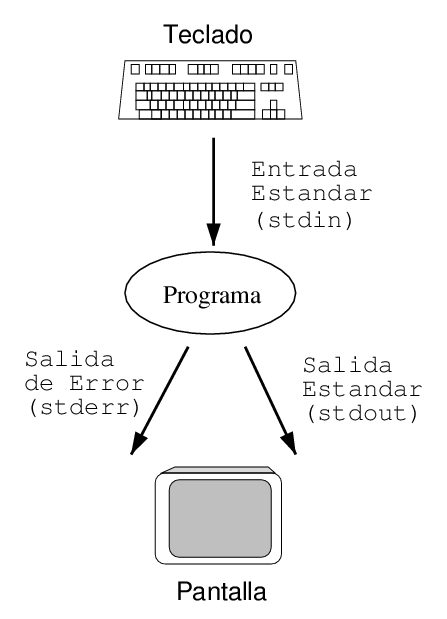
\includegraphics[width=4.2cm]{figs/stdinout}}
\end{figure}
\end{minipage} \hfill
\
\begin{minipage}{4cm}
\begin{itemize} 
\item entrada estándar
\item salida estándar
\item salida de error estándar
\end{itemize}
\end{minipage}\hfill
\end{frame}
%%---------------------------------------------------------------
\begin{frame}[fragile]
\frametitle{Paso de argumentos a órdenes}
Muchas órdenes se comportan así (no todas)
\begin{itemize} 
\item Sin argumentos: Entrada estándar\\ \texttt{ wc } 
\item 1 argumento: Nombre de fichero \\ \texttt{ wc fichero}
\item n nombres de fichero\\  \texttt{ wc fichero1 fichero2}
\end{itemize}
\end{frame}

%%---------------------------------------------------------------
\begin{frame}[fragile]
\begin{itemize} 
\item 
\texttt{cat}\\lee lo que hay en stdin y lo escribe en stdout \\
(Ctrl D: fin de fichero)
\item 
\texttt{cat fichero1 fichero2}\\lee los ficheros que se pasan como argumento y los escribe (concatenados) en stdout\\
(Ctrl D: fin de fichero)

\item 
\texttt{echo argumento}\\escribe en stdout el texto que se le pasa como argumento. Añade retorno de carro 
\item 
\texttt{echo -n argumento}\\escribe en stdout el texto que se le pasa como argumento
\item 
\texttt{less fichero}\\
escribe un fichero en stdout, permitiendo paginación

\end{itemize}
\end{frame}
%%---------------------------------------------------------------
\begin{frame}[fragile]
\frametitle{Redirecciones}
\begin{verbatim}
<    redirige stdin desde fichero
>    redirige stdout a fichero, reemplazando 
>>   redirige stdout a fichero, añadiendo
|    redirige stdout de un proceso a stdin del siguiente
\end{verbatim}
\begin{itemize} 
\item \texttt{cat }
\item \texttt{cat file1 file2 > file3}\\
 \texttt{cat file1 | less}\\
 \texttt{cat > file1}
\item 
 \texttt{ less fichero }\\
 \texttt{ cat fichero | less}\\
 \texttt{ less < fichero }\\
 (El resultado es el mismo, pero es importante distinguirlo)
\end{itemize}
\end{frame}



%%---------------------------------------------------------------
\begin{frame}[fragile]
1 representa stdout

2 representa stderr
\begin{itemize}
\item
\verb|mkdir /a/b/c 2> mi_fichero_errores |

Redirige stderr al fichero

\item
\verb|cp fichero_a fichero_b 2>/dev/null|

Redirige stderr al fichero \emph{sumidero} (Lo que se
copia en \verb|/dev/null| desaparece sin mostrarse)
\end{itemize}

Para escribir en 1 o en 2, es necesario anteponer \verb|&|
(para que no se confunda con un fichero que se llame \verb|"1"| o 
\verb|"2"|)
\begin{itemize}
\item
\verb|echo "ERROR: xxxx ha fallado"  >&2|

Redirige el mensaje a stderr
\end{itemize}

\verb|&| representa stdout y stderr

\begin{itemize}
\item
\verb|find /var  &>mi_fichero|
\end{itemize}

\end{frame}

%%---------------------------------------------------------------
\begin{frame}[fragile]
\frametitle{sudo y redirecciones}
La orden \emph{sudo} por omisión no incluye las posibles redirecciones
\begin{itemize}
\item
\verb|sudo echo hola > /tmp/aa|

El proceso \emph{echo} se lanza con la identidad del root  (id 0), 
pero la redirección la ejecuta el usuario ordinario


\item
Para poder usar redirecciones, ejecutamos una subshell con el parámetro -c

\verb|sudo bash -c  "echo hola>aa"|

\verb@sudo bash -c  "find /root | grep prueba "@


\end{itemize}

\end{frame}



%%---------------------------------------------------------------
\section{Programación de Scripts}
%%---------------------------------------------------------------


%%---------------------------------------------------------------
\begin{frame}[fragile]
\frametitle{Programación de Scripts}
\begin{itemize}
\item
En esta asignatura generalmente programaremos los scripts en python, que es más potente
y sencillo que bash
\item
Pero para tareas muy básicas (cp, mv, ln -s, etc) puede ser más
conveniente un script de bash
\end{itemize}

  \begin{footnotesize}
  \begin{verbatim}
#!/bin/bash
a="hola mundo"
echo $a 
  \end{verbatim}
  \end{footnotesize}

Para invocarlo:

  \begin{footnotesize}
  \begin{verbatim}
koji@mazinger:~$ ./holamundo 
hola mundo
  \end{verbatim}
  \end{footnotesize}

\end{frame}


%%---------------------------------------------------------------
\begin{frame}[fragile]
Es recomendable que un script empiece por \verb|#!/bin/bash|, pero
no es imprescindible

  \begin{footnotesize}
  \begin{verbatim}
a="hola mundo"
echo $a 
  \end{verbatim}
  \end{footnotesize}

En este caso podemos ejecutar una shell y pasarle como
primer argumento el fichero

  \begin{footnotesize}
  \begin{verbatim}
koji@mazinger:~$ bash holamundo 
hola mundo
  \end{verbatim}
  \end{footnotesize}

o bien ejecutar una shell y redirigir el fichero a su entrada estándar
  \begin{footnotesize}
  \begin{verbatim}
koji@mazinger:~$ bash <holamundo 
hola mundo
  \end{verbatim}
  \end{footnotesize}


Esto también puede ser útil para ejecutar un script sin permiso
de ejecución (basta el de lectura)

\end{frame}
%%---------------------------------------------------------------
\section{Filtros}
%%---------------------------------------------------------------

%%---------------------------------------------------------------
\begin{frame}[fragile]
\frametitle{Filtros}

\begin{itemize} 
\item
Los filtros son muy importantes en el scripting Unix:
grep, sed, sort, uniq, head, tail,  paste...
\item
Un mandato genera una salida, un filtro procesa la salida (selecciona filas o columnas, pega, reemplaza, cuenta,
ordena...) y lo pasa al siguiente mandato
\item


Ejemplo

\begin{footnotesize}
\begin{verbatim}
who | cut -c1-8 |sort |uniq | wc -l

ps -ef | grep miguel | grep -v gvim
\end{verbatim}
\end{footnotesize}



\item
En esta asignatura programaremos en python (de nivel más alto y más intuitivo), así que solo usaremos
filtros muy básicos
\end{itemize} 


\end{frame}
%%----------------------------------------------
\begin{frame}[fragile]
\frametitle{grep}

\begin{itemize} 
\item
grep es un filtro que selecciona las filas que contengan (o que no contengan) cierto patrón
\item
Para definir patrones de texto, emplea expresiones regulares (regexp)
\begin{itemize} 
\item
Las regexp de grep, sed y awk son \emph{clásicas}. 
\item
Las regexp de perl, python y ruby son una evolución de las regexp clásicas. Son mucho más intuitivas
\item
Para tareas muy sencillas, podemos usar grep o sed. Si nuestras necesidades son más complejas y podemos
elegir qué herramienta usar, mejor python (o ruby)
\end{itemize}
\end{itemize}

\end{frame}
%%----------------------------------------------
\begin{frame}[fragile]

grep con un argumento
\begin{itemize} 
\item
\verb|grep <patrón> | 

Lee stdin y escribe en stdout las líneas que encajen en el patrón
\item
\verb|grep -v <patrón> | 

Lee stdin y escribe en stdout las líneas que \textbf{no} encajen en el patrón
\item
\verb|grep -i <patrón> | 

Lee stdin y escribe en stdout las líneas que encajen en el patrón, ignorando mayúsculas/minúsculas

\end{itemize} 


Ejemplos
  \begin{footnotesize}
  \begin{verbatim}
ps -ef | grep -i ejemplo
ps -ef | grep -v jperez
dmesg | grep eth
  \end{verbatim}
  \end{footnotesize}

\end{frame}
%%----------------------------------------------
\begin{frame}[fragile]

grep con dos o más argumentos

\begin{itemize} 
\item
\verb|grep <patrón> <fichero_1> ... <fichero_n> | 

Lee los ficheros 
indicados
%\verb|<fichero_1> ... <fichero_n>| 
y escribe en stdout las líneas que encajen
en el patrón
\end{itemize}



Ejemplos
  \begin{footnotesize}
  \begin{verbatim}
grep linux *.txt
grep -i hidalgo quijote.txt
grep -v 193.147 /etc/hosts
  \end{verbatim}
  \end{footnotesize}

Atención: Si el patrón a buscar incluye espacios, es necesario escribirlo entre comillas.
  \begin{footnotesize}
\begin{itemize} 
\item 
\verb|grep "la mancha" quijote.txt  |  

Busca el patrón \emph{la mancha} en el fichero \emph{quijote.txt}
\item 
\verb|grep la mancha quijote.txt  |  

Busca el patrón \emph{la} en el fichero \emph{mancha} y en el fichero \emph{quijote.txt} 

\end{itemize}
  \end{footnotesize}

\end{frame}


%%---------------------------------------------------------------
\begin{frame}[fragile]
\textcolor{red}{Atención}: 
\begin{itemize}
\item
Hablamos de patrones, no de palabras.
El patrón \emph{ana} encaja en la palabra
\emph{ana}
pero también en
\emph{rosana}
\item
Los metacaracteres de las regexp no son iguales que los metacaracteres (comodines) del bash
\end{itemize}

Algunos metacaracteres:
\begin{itemize}
\item
\begin{verbatim}
grep -i '\<ana\>'
\end{verbatim}
Principio de palabra, patrón \emph{ana}, final de palabra. Insensible a mayúsculas.
(Dicho de otro modo, la palabra \emph{ana},
sin confusión con \emph{Mariana})
\item
\begin{verbatim}
grep -i '\<ana p.rez\>'
\end{verbatim}

El punto representa cualquier carácter (equivalente a la interrogación en las shell de bash)
\item
\begin{verbatim}
grep -i '\<ana p[eé]rez\>'
\end{verbatim}

Después de la \emph{p} puede haber una \emph{e} con tilde o sin tilde

\end{itemize}


\end{frame}
%%---------------------------------------------------------------
\begin{frame}[fragile]
\frametitle{xargs}

Mediante pipes podemos formar filtros concatenando órdenes.
Pero ¿qué sucede cuando la información la necesitamos como
parámetro, no en la entrada estándar?

  \begin{footnotesize}
  \begin{verbatim}
locate -i basura | rm    # ¡Esto NO FUNCIONA!
  \end{verbatim}
  \end{footnotesize}

Podemos usar la orden xargs

  \begin{footnotesize}
  \begin{verbatim}
locate -i basura | xargs rm
  \end{verbatim}
  \end{footnotesize}

Ejecuta rm tantas veces como líneas haya en stdin. Y le pasa cada línea
como argumento


\end{frame}

%%----------------------------------------------
\begin{frame}[fragile]


\begin{itemize}
\item

Cuando necesitamos que la línea de entrada vaya en una posición
distinta, usamos la opción \verb|-I replstr| , donde \verb|replstr| es la 
\emph{replace string},
la cadena que reemplazaremos por el argumento
\item

El valor recomendado es 
\verb|{}|,
porque no es fácil que aparezca en otro sitio
\end{itemize}

  \begin{footnotesize}
  \begin{verbatim}
locate  basura | xargs -I {} mv {} /tmp/papelera
find . | grep -i jpg | xargs -I {} mv {} /tmp/fotos
  \end{verbatim}
  \end{footnotesize}

\end{frame}








%%---------------------------------------------------------------
\section{Manejo básico de procesos}
%%---------------------------------------------------------------

\begin{frame}[fragile]
\frametitle{Manejo básico de procesos}
\begin{itemize} 
\item \verb|ps       | Información sobre los procesos \\
\verb|ps  -e   | Información sobre todos los procesos de la maquina\\
\verb|ps  -ef  | Formato largo\\

\item \verb|top      | Muestra los procesos que consumen más cpu
\item \verb|kill     | Envia una señal a un proceso
%\item CTRL+C    \\Señal SIGINT
%\item CTRL+Z   Detiene proceso
%\item CTRL+D    \\Fin de fichero
\end{itemize}
\end{frame}


%--------------------------------------------------------------------


\begin{frame}[fragile]
\frametitle{Señales}
La orden kill envía señales a procesos

\verb|kill [señal] [proceso]|
\begin{itemize}
\item
15 SIGTERM (valor por defecto) 
\item
9  SIGKILL  
\item
2  SIGINT (Ctrl C) Lo envia tty a todos los programas que se estén ejecutando
en primer plano en el terminal, y a todos los programas lanzados por estos.
\item
19  SIGSTOP (Ctrl Z) Detiene
\item
18 SIGCONT Continua si estaba detenido

%\item
%3  SIGQUIT    señal para "haz un core"
%\item
%1  SIGHUP
\end{itemize}

Las señales SIGKILL y SIGSTOP no se pueden ignorar ni bloquear

\end{frame}

%%----------------------------------------------
\begin{frame}[fragile]

Ejemplos:
      
\verb|kill -9 2341|

\verb|kill -sigstop 49322|

Tabla con las señales: 

\verb|man 7 signal|
\end{frame}


% poner ejemplo con tictac, no con xcalc (que es la práctica) ni con
% top (que es un lio) ni con vmstat (que lo explicas luego
% en control de tareas)



%%---------------------------------------------------------------
%\begin{frame}[fragile]
%\frametitle{Ejemplo de SIGINT}
%Sea un script llamado \emph{mitop}
%  \begin{footnotesize}
%  \begin{verbatim}
%#!/bin/bash
%top
%  \end{verbatim}
%  \end{footnotesize}
%
%Si enviamos a \emph{mitop} la señal...
%\begin{itemize}
%\item
%SIGTERM, el proceso \emph{mitop} morirá, pero \verb|top|, no
%\item
%SIGINT, ambos procesos morirán
%\end{itemize}
%
%\end{frame}


%%---------------------------------------------------------------
\begin{frame}[fragile]
\begin{itemize}
\item
Una manera típica de localizar un proceso \emph{a mano}  es
\verb$ps -ef | grep <cadena>$

o

\verb$ps -ef | grep <cadena> | less$
\item
\verb|killall| envía señales a procesos a partir de su nombre. (El nombre de la señal 
se indica de manera ligeramente distinta a como se emplea en kill)
\item
\verb|pkill| envía señales a procesos, identificables mediante nombre u otros atributos

\end{itemize}

\end{frame}



%%---------------------------------------------------------------
%\begin{frame}[fragile]
%\subsection{Multiusuario}
%\begin{itemize}        
%\item whoami
%\item hostname
%\item who
%\item id
%\item finger
%\end{itemize}
%\end{frame}



\end{document}
%-------------------------------------END DOCUMENT






\begin{frame}[fragile]
  \section{Inicio de sesión}
{\flushleft\fontsize{8pt}{8pt}\selectfont
\verb|Debian GNU/Linux 3.1 blas tty1|\\
\verb| |\\
\verb|blas login: |\texttt{\textbf{cespedes}}\\
\verb|Password:|\\
\verb| |\\
\verb|Last login: Sat Jan 29 17:25:03 2005 on tty4|\\
\verb| |\\
\verb|cespedes@blas:~$ |\texttt{\textbf{id}}\\
\verb|uid=1000(cespedes) gid=1000(cespedes) groups=20(dialout),24(cdrom),|\\
\verb|25(floppy),29(audio),44(video),1000(cespedes)|\\
\verb|cespedes@blas:~$ |\texttt{\textbf{su}}\\
\verb|Password:|\\
\verb|blas:/home/cespedes# |\texttt{\textbf{id}}\\
\verb|uid=0(root) gid=0(root) groups=0(root)|\\
\verb|blas:/home/cespedes# |\texttt{\textbf{exit}}\\
\verb|exit|\\
\verb|cespedes@blas:~$ |\texttt{\textbf{id}}\\
\verb|uid=1000(cespedes) gid=1000(cespedes) groups=20(dialout),24(cdrom),|\\
\verb|25(floppy),29(audio),44(video),1000(cespedes)|\\
}
\end{frame}

\begin{frame}[fragile]
  \section{El intérprete de órdenes}
  El intérprete, o \emph{shell}, es el programa encargado de
  leer las órdenes dadas por un usuario y ejecutarlas una a una

  Hay muchas \emph{shell}s distintas. Hoy en día, la más común es \texttt{bash}.
  \begin{itemize}
    \item Órdenes internas: control de la shell y programación:\\
	    \texttt{cd}, \texttt{echo}, \texttt{exit}, \texttt{if}, \texttt{for}, \texttt{while}, \texttt{break}, \texttt{return}\ldots
    \item Órdenes externas: ejecución de otro programa
    \item Variables: comienzan con \verb+$+.\\
	    Predefinidas: \verb+$HOME+, \verb+$PATH+, \verb+$$+\ldots\\
	    \verb+cespedes@blas:~$ +\texttt{\textbf{echo \$PATH}}\\
	    \verb+/home/cespedes/bin:/usr/local/bin:/usr/bin:+\\
	    \verb+/bin:/usr/bin/X11:/usr/games+
  \end{itemize}
\end{frame}

\begin{frame}[fragile]
  \section{Páginas de manual}
  \texttt{\$ \textbf{man} \emph{[sección] página}} \hspace{\fill} (\texttt{\textbf{man} \emph{sección} \textbf{intro}})
  \begin{itemize}
    \item[]\textbf{Sección 1.} Órdenes de usuario
    \item[]\textbf{Sección 2.} Llamadas al sistema
    \item[]\textbf{Sección 3.} Llamadas a funciones de biblioteca
    \item[]\textbf{Sección 4.} Ficheros especiales
    \item[]\textbf{Sección 5.} Ficheros, formatos y protocolos
    \item[]\textbf{Sección 6.} Juegos
    \item[]\textbf{Sección 7.} Convenciones, miscelánea
    \item[]\textbf{Sección 8.} Órdenes de administrador y privilegiadas
  \end{itemize}
\end{frame}

\begin{frame}[fragile]
  \section{Operaciones con ficheros: consulta}
  \begin{itemize}
    \item \texttt{pwd}$^*$ $\rightarrow$ Indica cuál es el directorio actual
    \item \texttt{cd}$^*$ $\rightarrow$ Cambia el directorio actual
    \item \texttt{ls} $\rightarrow$ Muestra el contenido de un directorio
    \item \texttt{cat} $\rightarrow$ Muestra el contenido de un fichero
    \item \texttt{find} $\rightarrow$ Busca ficheros que cumplan
          determinadas catacterísticas
    \item \texttt{du} $\rightarrow$ Indica el tamaño de un fichero
    \item \texttt{cmp} $\rightarrow$ Compara dos ficheros
    \item \texttt{diff} $\rightarrow$ Muestra diferencias entre dos ficheros
  \end{itemize}
\end{frame}

\begin{frame}[fragile]
  \section{Operaciones con ficheros: creación, borrado}
  \begin{itemize}
    \item \texttt{cp} $\rightarrow$ Copia un fichero en otro destino
    \item \texttt{mv} $\rightarrow$ Renombra un fichero y/o lo mueve
          de un directorio a otro
    \item \texttt{ln} $\rightarrow$ Crea un enlace de un fichero a otro
    \item \texttt{rm} $\rightarrow$ Borra un fichero
    \item \texttt{rmdir} $\rightarrow$ Borra un directorio
    \item \texttt{mkdir} $\rightarrow$ Crea un directorio
    \item \texttt{mknod}$^*$ $\rightarrow$ Crea un fichero ``especial''
    \item \texttt{tar} $\rightarrow$ Manipula conjuntos de ficheros
    \item \texttt{gzip} $\rightarrow$ Comprime un fichero
  \end{itemize}
\end{frame}

\begin{frame}[fragile]
  \section{Operaciones con ficheros: manipulación}
  \begin{itemize}
    \item \texttt{touch} $\rightarrow$ Modifica la fecha de última
          modificación de un fichero
    \item \texttt{chmod} $\rightarrow$ Cambia los permisos de acceso
          a un fichero
    \item \texttt{chown}$^*$ $\rightarrow$ Cambia el dueño de un fichero
    \item \texttt{chgrp}$^*$ $\rightarrow$ Cambia el grupo de un fichero
  \end{itemize}
\end{frame}

\begin{frame}[fragile]
  \section{Manejo de ficheros de texto}
  \begin{itemize}
    \item Editores: \texttt{ed}, \texttt{vi} (\texttt{vim}, \texttt{elvis},
		    \texttt{nvi}), \texttt{emacs} (\texttt{xemacs},
		    \texttt{jove}), \texttt{gedit}, \texttt{kedit},
		    \texttt{nano}, \texttt{jed}, \texttt{wily},
		    \texttt{the}, \texttt{aee}\ldots
    \item Búsqueda de cadenas: \texttt{grep}
{\flushleft\fontsize{6pt}{6pt}\selectfont
\verb|cespedes@blas:~$ |\texttt{\textbf{grep Debian /etc/motd}}\\
\verb|The programs included with the Debian GNU/Linux system are free software;|\\
\verb|Debian GNU/Linux comes with ABSOLUTELY NO WARRANTY, to the extent|\\
}
    \item Sustitución de cadenas: \texttt{sed}
{\flushleft\fontsize{6pt}{6pt}\selectfont
\verb|cespedes@blas:~$ |\texttt{\textbf{grep Debian /etc/motd | sed s/GNU/Ñu/}}\\
\verb|The programs included with the Debian Ñu/Linux system are free software;|\\
\verb|Debian Ñu/Linux comes with ABSOLUTELY NO WARRANTY, to the extent|\\
}
    \item Manipulación general: \texttt{awk}
  \end{itemize}
\end{frame}

\begin{frame}[fragile]
  \section{Usuarios conectados}
{\flushleft\fontsize{8pt}{8pt}\selectfont
\verb|cespedes@blas:~$ |\texttt{\textbf{who}}\\
\verb|rover    pts/0        Feb 16 09:14 (:0.0)|\\
\verb|cespedes pts/1        Feb 16 10:56 (:0.0)|\\
\verb|cespedes@blas:~$ |\texttt{\textbf{who am i}}\\
\verb|cespedes pts/1        Feb 16 10:56 (:0.0)|\\
\verb|cespedes@blas:~$ |\texttt{\textbf{tty}}\\
\verb|/dev/pts/1|\\
\verb|cespedes@blas:~$ |\texttt{\textbf{finger}}\\
\verb|Login     Name               Tty      Idle  Login Time   Office|\\
\verb|rover     Roberto Lumbreras  pts/0    1:59  Feb 16 09:14 (:0.0)|\\
\verb|cespedes  Juan Cespedes      pts/1          Feb 16 10:56 (:0.0)|\\
\verb|cespedes@blas:~$ |\texttt{\textbf{w}}\\
\verb| 10:56:15 up 18:12,  2 users,  load average: 0,00, 0,12, 0,22|\\
\verb|USER     TTY      FROM              LOGIN@   IDLE   JCPU   PCPU WHAT|\\
\verb|rover    pts/0    :0.0             09:14    1:59m  0.02s  0.02s -bash|\\
\verb|cespedes pts/1    :0.0             10:56    0.00s  0.03s  0.01s w|\\
\verb|cespedes@blas:~$|\\}
\end{frame}

\begin{frame}[fragile]
  \section{Procesos}
{\flushleft\fontsize{8pt}{8pt}\selectfont
\verb|cespedes@blas:~$ |\texttt{\textbf{ps}}\\
\verb|  PID TTY          TIME CMD|\\
\verb| 3086 pts/1    00:00:00 bash|\\
\verb| 3087 pts/1    00:00:00 ps|\\
\verb|cespedes@blas:~$ |\texttt{\textbf{ps f}}\\
\verb|  PID TTY      STAT   TIME COMMAND|\\
\verb| 3086 pts/1    Ss     0:00 -bash|\\
\verb| 3088 pts/1    R+     0:00  \_ ps f|\\
\verb+cespedes@blas:~$ +\texttt{\textbf{ps af}}\\
\verb|  PID TTY      STAT   TIME COMMAND|\\
\verb|  623 tty1     Ss+    0:00 /sbin/getty 38400 tty1|\\
\verb|  624 tty2     Ss+    0:00 /sbin/getty 38400 tty2|\\
\verb|  625 tty3     Ss+    0:00 /sbin/getty 38400 tty3|\\
\verb|  626 tty4     Ss+    0:00 /sbin/getty 38400 tty4|\\
\verb|  627 tty5     Ss+    0:00 /sbin/getty 38400 tty5|\\
\verb|  628 tty6     Ss+    0:00 /sbin/getty 38400 tty6|\\
\verb| 2812 pts/0    Ss+    0:00 -bash|\\
\verb| 3086 pts/1    Ss     0:00 -bash|\\
\verb| 3282 pts/1    R+     0:00  \_ ps af|\\}
\end{frame}

\begin{frame}[fragile]
  \section{Procesos (2)}
{\flushleft\fontsize{7pt}{7pt}\selectfont
\verb|cespedes@blas:~$ |\texttt{\textbf{top}}\\
\verb|top - 11:55:44 up 18:52, 31 users,  load average: 0.49, 0.31, 0.25|\\
\verb|Tasks: 177 total,   3 running, 174 sleeping,   0 stopped,   0 zombie|\\
\verb|Cpu(s): 11.8% us,  2.9% sy,  0.0% ni, 85.3% id,  0.0% wa,  0.0% hi,  0.0% si|\\
\verb|Mem:   1035924k total,   687348k used,   348576k free,    89188k buffers|\\
\verb|Swap:  2457904k total,        0k used,  2457904k free,   292060k cached|\\
\verb||\\
\verb|  PID USER      PR  NI  VIRT  RES  SHR S %CPU %MEM    TIME+  COMMAND           |\\
\verb|12118 cespedes  15   0  9500 2964 2640 S  8.7  0.3   0:04.92 mpg123             |\\
\verb|12806 cespedes  16   0  2188 1128  848 R  8.7  0.1   0:00.10 top                |\\
\verb|15888 cespedes  15   0  5824 3184 2212 S  2.9  0.3   0:00.30 xterm              |\\
\verb|    1 root      16   0  1500  516  456 S  0.0  0.0   0:00.44 init               |\\
\verb|    2 root      34  19     0    0    0 S  0.0  0.0   0:00.06 ksoftirqd/0        |\\
\verb|    3 root       5 -10     0    0    0 S  0.0  0.0   0:04.20 events/0           |\\
\verb|    4 root       5 -10     0    0    0 S  0.0  0.0   0:00.00 khelper            |\\
\verb|   16 root       5 -10     0    0    0 S  0.0  0.0   0:00.00 kacpid             |\\
\verb|  107 root       5 -10     0    0    0 S  0.0  0.0   0:00.07 kblockd/0          |\\
\verb|  138 root      20   0     0    0    0 S  0.0  0.0   0:00.00 pdflush            |\\
\verb|  139 root      15   0     0    0    0 S  0.0  0.0   0:00.15 pdflush            |\\
\verb|  141 root      15 -10     0    0    0 S  0.0  0.0   0:00.00 aio/0              |\\
\verb|  140 root      17   0     0    0    0 S  0.0  0.0   0:00.82 kswapd0            |\\
\verb|  728 root      15   0     0    0    0 S  0.0  0.0   0:00.00 kseriod            |\\
}
\end{frame}

\begin{frame}[fragile]
  \section{Procesos (3)}
  \begin{itemize}
    \item Pausa en un proceso: \texttt{sleep}
    \item Terminación y avisos a procesos: \texttt{kill}
  \end{itemize}
  \vspace{.1cm}
{\flushleft\fontsize{8pt}{8pt}\selectfont
\verb|cespedes@blas:~$ |\texttt{\textbf{sleep 3600 \&}}\\
\verb|[1] 17093|\\
\verb|cespedes@blas:~$ |\texttt{\textbf{kill -l}}\\
\verb| 1) SIGHUP       2) SIGINT       3) SIGQUIT      4) SIGILL|\\
\verb| 5) SIGTRAP      6) SIGABRT      7) SIGBUS       8) SIGFPE|\\
\verb| 9) SIGKILL     10) SIGUSR1     11) SIGSEGV     12) SIGUSR2|\\
\verb|13) SIGPIPE     14) SIGALRM     15) SIGTERM     17) SIGCHLD|\\
\verb|18) SIGCONT     19) SIGSTOP     20) SIGTSTP     21) SIGTTIN|\\
\verb|22) SIGTTOU     23) SIGURG      24) SIGXCPU     25) SIGXFSZ|\\
\verb|26) SIGVTALRM   27) SIGPROF     28) SIGWINCH    29) SIGIO|\\
\verb|30) SIGPWR      31) SIGSYS      33) SIGRTMIN    34) SIGRTMIN+1|\\
\verb|cespedes@blas:~$ |\texttt{\textbf{kill -6 17093}}\\
\verb|[1]+ Aborted                  sleep 3600|\\
\verb|cespedes@blas:~$ |\\
}
\end{frame}

\begin{frame}[fragile]
  \section{Herramientas de gestión de discos}
  \begin{itemize}
    \item \texttt{fdisk} $\rightarrow$ Muestra y modifica la tabla
          de particiones de un disco
    \item \texttt{mkfs} $\rightarrow$ Crea un sistema de ficheros
          (\emph{formatea} una partición)
    \item \texttt{fsck} $\rightarrow$ Comprueba la integridad de un
          sistema de ficheros
    \item \texttt{df} $\rightarrow$ Muestra tablas de montaje y uso
          de cada partición
    \item \texttt{mount} $\rightarrow$ Muestra tablas de montaje,
          monta una partición
    \item \texttt{umount} $\rightarrow$ Desmonta una partición
  \end{itemize}
\end{frame}

\begin{frame}[fragile]
  \section{Herramientas de gestión de memoria}
  \begin{itemize}
    \item \texttt{top} $\rightarrow$ Información general acerca de
          los procesos del sistema y de su uso de memoria y de CPU
    \item \texttt{free} $\rightarrow$ Resumen del estado de la memoria
          en el sistema
{\flushleft\fontsize{6pt}{6pt}\selectfont
\verb|cespedes@blas:~$ |\texttt{\textbf{free}}\\
\verb|             total       used       free     shared    buffers     cached|\\
\verb|Mem:       1035924     735480     300444          0      94620     333940|\\
\verb|-/+ buffers/cache:     306920     729004|\\
\verb|Swap:      2457904          0    2457904|\\
}
  \end{itemize}
  Gestión del \emph{swap} (área de intercambio):
  \begin{itemize}
    \item \texttt{mkswap} $\rightarrow$ Crea un área de intercambio
    \item \texttt{swapon} $\rightarrow$ Activa un área de intercambio
    \item \texttt{swapoff} $\rightarrow$ Desactiva un área de intercambio
  \end{itemize}
\end{frame}

\begin{frame}[fragile]
  \section{Gestión de red (TCP/IP)}
  \begin{itemize}
    \item \texttt{ifconfig} $\rightarrow$ Muestra/modifica información
          de las tarjetas de red del sistema
{\flushleft\fontsize{6pt}{6pt}\selectfont
\verb|root@orion:~$ |\texttt{\textbf{ifconfig eth0}}\\
\verb|eth0      Link encap:Ethernet  HWaddr 00:0D:9D:D1:6A:27  |\\
\verb|          inet addr:193.147.71.90  Bcast:193.147.71.255  Mask:255.255.255.128|\\
\verb|          UP BROADCAST RUNNING MULTICAST  MTU:1500  Metric:1|\\
\verb|          RX packets:2219198 errors:0 dropped:0 overruns:0 frame:0|\\
\verb|          TX packets:949209 errors:0 dropped:0 overruns:0 carrier:0|\\
\verb|          collisions:0 txqueuelen:1000 |\\
\verb|          RX bytes:553335922 (527.7 MiB)  TX bytes:357891938 (341.3 MiB)|\\
}
    \item \texttt{route} $\rightarrow$ Muestra/modifica información
          de la tabla de rutas del sistema
{\flushleft\fontsize{6pt}{6pt}\selectfont
\verb|root@orion:~$ |\texttt{\textbf{route}}\\
\verb|Kernel IP routing table|\\
\verb|Destination     Gateway         Genmask         Flags Metric Ref    Use Iface|\\
\verb|10.3.0.2        *               255.255.255.255 UH    0      0        0 tun0|\\
\verb|193.147.71.0    *               255.255.255.128 U     0      0        0 eth0|\\
\verb|192.168.64.0    *               255.255.255.0   U     0      0        0 eth1|\\
\verb|default         193.147.71.1    0.0.0.0         UG    0      0        0 eth0|\\
}
  \end{itemize}
\end{frame}

\begin{frame}[fragile]
  \section{Gestión de red (TCP/IP) (2)}
  \begin{itemize}
    \item \texttt{netstat} $\rightarrow$ Muestra el estado de las conexiones
          TCP/IP de la máquina
{\flushleft\fontsize{6pt}{6pt}\selectfont
\verb|root@orion:~$ |\texttt{\textbf{netstat -nt}}\\
\verb|Active Internet connections (w/o servers)|\\
\verb|Proto Recv-Q Send-Q Local Address           Foreign Address         State      |\\
\verb|tcp        0      0 193.147.71.90:137       193.147.62.27:32887     ESTABLISHED|\\
\verb|tcp        0      0 193.147.71.90:36054     193.147.71.88:80        TIME_WAIT|\\
\verb|tcp6       0     48 ::ffff:193.147.71.90:22 ::ffff:193.147.62:33050 ESTABLISHED|\\
\verb|tcp6       0      0 ::ffff:193.147.71.90:22 ::ffff:193.147.62:32983 ESTABLISHED|\\
}
  \end{itemize}
  Información acerca de protocolos, servicios, puertos, etc. en los ficheros
\texttt{/etc/protocols} y \texttt{/etc/services}
\end{frame}



\end{document}




\end{document}


